\documentclass[bibtotoc,liststotoc,BCOR=5mm,DIV=12]{article}

% use this declaration to set specific page margins
%\usepackage[a4paper , lmargin = {2.7cm} , rmargin = {2.9cm} , tmargin = {2.7cm} , bmargin = {4.6cm} ]{geometry}
\usepackage[a4paper]{geometry}

\setlength{\parskip}{\baselineskip}%
\setlength{\parindent}{0pt}
\usepackage[ngerman, english]{babel}
\usepackage{bibgerm}
\usepackage[section]{placeins}
\usepackage[T1]{fontenc} % german characters

\usepackage{helvet} % Include the helvet package
\renewcommand{\rmdefault}{phv} % Helvetica for the main text
\renewcommand{\sfdefault}{phv} % Helvetica for sans-serif

\usepackage{graphicx} 				% it's recommended to use PDF images but you can use JPG or PNG as well
\usepackage{url}           		% format URLs
\usepackage[hidelinks]{hyperref} 				% create hyperlinks
\usepackage{listings, color}	% for source code
% two figures next to each other (example: figure 3a), figure 3b)
\usepackage{scrlayer-scrpage}					% header and footer line
\usepackage{todonotes}
\usepackage{setspace}
\usepackage{caption}
\usepackage{subcaption}
\usepackage{amssymb}
\usepackage{amsmath}
\usepackage{booktabs}
\usepackage{multirow}
\usepackage{siunitx}
\usepackage{float}
% header and footer line - no header & footer line on pages where a new chapter starts
\captionsetup{labelfont=bf}
\pagestyle{scrheadings}
\automark[subsection]{section}
\ohead{\headmark}
\ihead{Heng Zhang}
\ofoot[]{\thepage}
\onehalfspacing

% set path where images are stored
\graphicspath{{./img/}}


\begin{document}
% ---------------------------------------------------------------
    \thispagestyle{empty}
\begin{center}

\vspace*{1cm}

\includegraphics[width=4cm]{tu_logo}
\vspace*{0.5cm}

{\LARGE \textbf{Technische Universität Berlin}}\\
\vspace*{0.3cm}
Faculty V – Mechanical Engineering and Transport Systems\\
Institute for Machine Design and System Technology\\
Chair of Cyber-Physical Systems in Mechanical Engineering\\

\vspace*{2cm}

{\LARGE Master Thesis}\\

\vspace{1.0cm}
{\LARGE \textbf{Comparative Analysis of Reservoir Computing}}\\
\vspace*{0.3cm}
{\LARGE \textbf{and LSTM Networks for Chaotic Time-Series Prediction}}\\
\vspace*{1.0cm}


Heng Zhang\\
M.Sc. Mechanical Engineering\\
Matriculation Number: 463983\\
Berlin, February 2026\\
\vspace*{1.0cm}

Supervised by\\
Prof. Dr. Merten Stender\\


\vspace*{0.5cm}
Assistant Supervisor\\
Dr. Manish Yadav
\vspace{3cm}


\end{center}


    \thispagestyle{empty}
    \clearpage
    
    
    \thispagestyle{empty}

\section*{Eigenständigkeitserklärung}

\begin{large}

\vspace*{4cm}

\noindent
Hiermit versichere ich, dass ich die vorliegende Arbeit eigenständig ohne Hilfe Dritter und ausschließlich unter Verwendung der
aufgeführten Quellen und Hilfsmittel angefertigt habe. Alle Stellen die den benutzten Quellen und Hilfsmitteln unverändert oder
sinngemäß entnommen sind, habe ich als solche kenntlich gemacht. Sofern generative KI-Tools verwendet wurden, habe ich Produktnamen, Hersteller, die jeweils verwendete Softwareversion und die jeweiligen Einsatzzwecke (z.B. sprachliche Überprüfung und Verbesserung der Texte, systematische Recherche) benannt.
Ich verantworte die Auswahl, die Übernahme und sämtliche Ergebnisse des von mir verwendeten KI-generierten Outputs vollumfänglich selbst.
\vspace{2cm}

\noindent
Berlin, den xx.xx.xxx

\vspace{3cm}

\hspace*{7cm}%
\dotfill\\
\hspace*{8.5cm}%
(Unterschrift)

\end{large}
 
    \thispagestyle{empty}
    \clearpage
    
    
    \thispagestyle{empty}
\vspace*{1.0cm}

\begin{center}
    \textbf{Abstract}
\end{center}

\vspace*{0.5cm}

\noindent
Data-driven approaches have become essential for modeling and forecasting nonlinear dynamical systems. Long Short-Term Memory (LSTM) networks are widely used for sequence prediction due to their ability to capture temporal dependencies, but they typically require large datasets and numerous trainable parameters, resulting in significant computational and environmental costs. Reservoir Computing (RC), particularly Echo-State Networks (ESNs), offers a lightweight alternative where only the output layer is trained, enabling faster learning and robust generalization with limited data. However, a systematic comparison between these paradigms under matched model capacity and data availability remains underexplored.

\noindent
This thesis presents a quantitative comparison of Echo-State Networks (ESNs), implemented using the pyReCo library, and LSTM architectures on three canonical chaotic time-series benchmarks: the Lorenz system, the Mackey-Glass system, and the Santa Fe laser dataset. Both model families are evaluated under matched total parameter budgets (small: ${\sim}1$K, medium: ${\sim}10$K, large: ${\sim}50$K parameters) and varying training data sizes (1\,000--10\,000 samples). Performance is assessed using prediction accuracy (MSE, R\textsuperscript{2}), computational efficiency, and sustainability metrics across 417 experiments with five random seeds each. Statistical significance is established through paired t-tests and Wilcoxon signed-rank tests with Cohen's d effect sizes.

\noindent
The results reveal a strongly dataset-dependent outcome: ESNs achieve near-perfect predictions on chaotic synthetic systems (Lorenz: R\textsuperscript{2}\,$=$\,0.999, Mackey-Glass: R\textsuperscript{2}\,$=$\,0.987), significantly outperforming LSTM (R\textsuperscript{2}\,$=$\,0.825 and 0.942, respectively) with $p < 0.001$. Conversely, LSTM dominates on the real-world Santa Fe laser dataset (R\textsuperscript{2}\,$=$\,0.934 vs.\ 0.770, $p < 0.001$). ESNs are up to 40$\times$ faster to train at small parameter budgets, while LSTM becomes faster at large budgets. All significant differences exhibit large effect sizes (Cohen's d\,$>$\,2.0). These findings demonstrate that model selection for chaotic time-series prediction should be guided by dataset characteristics rather than architectural preference, and highlight Reservoir Computing as a computationally efficient alternative for well-characterized dynamical systems.

\vspace{0.5cm}
\noindent\textbf{AI Tool Disclosure:} This thesis was developed with the assistance of Claude Code (Anthropic, model: Claude Opus 4). The tool was used for implementing experiment scripts (Python), drafting and revising LaTeX text, generating figures from experimental data, and supporting literature research. All AI-generated content was reviewed, revised, and validated by the author. The scientific conception, experimental design, interpretation of results, and final editing were conducted independently.


    \thispagestyle{empty}
    \clearpage
    
    \thispagestyle{empty}
\vspace*{0.2cm}

\begin{center}
    \textbf{Zusammenfassung}
\end{center}

\vspace*{0.5cm}

\noindent
Datengetriebene Methoden sind für die Modellierung und Vorhersage nichtlinearer dynamischer Systeme unverzichtbar geworden. Long Short-Term Memory (LSTM) Netzwerke werden aufgrund ihrer Fähigkeit, zeitliche Abhängigkeiten zu erfassen, häufig für Sequenzvorhersagen eingesetzt. Sie erfordern jedoch typischerweise große Datensätze und zahlreiche trainierbare Parameter, was zu erheblichen Rechen- und Umweltkosten führt. Reservoir Computing (RC), insbesondere Echo-State Networks (ESNs), bietet eine ressourcenschonende Alternative, bei der nur die Ausgangsschicht trainiert wird, was schnelleres Lernen und robuste Generalisierung bei begrenzten Daten ermöglicht. Ein systematischer Vergleich dieser Paradigmen unter gleichen Modellkapazitäten und Datenverfügbarkeiten wurde bisher jedoch kaum untersucht.

\noindent
Diese Arbeit präsentiert einen quantitativen Vergleich von Echo-State Networks (ESNs), implementiert mit der pyReCo-Bibliothek, und LSTM-Architekturen auf drei kanonischen chaotischen Zeitreihen-Benchmarks: dem Lorenz-System, dem Mackey-Glass-System und dem Santa-Fe-Laser-Datensatz. Beide Modellfamilien werden unter gleichen Gesamtparameterbudgets (klein: ${\sim}1$K, mittel: ${\sim}10$K, groß: ${\sim}50$K Parameter) und variierenden Trainingsdatengrößen (1\,000--10\,000 Datenpunkte) evaluiert. Die Leistung wird anhand von Vorhersagegenauigkeit (MSE, R\textsuperscript{2}), Recheneffizienz und Nachhaltigkeitsmetriken über 417 Experimente mit jeweils fünf zufälligen Seeds bewertet. Die statistische Signifikanz wird durch gepaarte t-Tests und Wilcoxon-Vorzeichen-Rang-Tests mit Cohens d Effektstärken ermittelt.

\noindent
Die Ergebnisse zeigen ein stark datensatzabhängiges Bild: ESNs erreichen nahezu perfekte Vorhersagen auf chaotischen synthetischen Systemen (Lorenz: R\textsuperscript{2}\,$=$\,0,999, Mackey-Glass: R\textsuperscript{2}\,$=$\,0,987) und übertreffen LSTM signifikant (R\textsuperscript{2}\,$=$\,0,825 bzw.\ 0,942, $p < 0{,}001$). Umgekehrt dominiert LSTM auf dem realen Santa-Fe-Laser-Datensatz (R\textsuperscript{2}\,$=$\,0,934 vs.\ 0,770, $p < 0{,}001$). ESNs sind bei kleinen Parameterbudgets bis zu 40$\times$ schneller zu trainieren, während LSTM bei großen Budgets schneller wird. Alle signifikanten Unterschiede weisen große Effektstärken auf (Cohens d\,$>$\,2,0). Diese Ergebnisse zeigen, dass die Modellwahl für chaotische Zeitreihenvorhersagen von den Datensatzeigenschaften abhängen sollte, und heben Reservoir Computing als recheneffiziente Alternative für gut charakterisierte dynamische Systeme hervor.
    \thispagestyle{empty}
    
    
    \tableofcontents
    \thispagestyle{empty}
    \newpage

    
    \listoffigures
    \thispagestyle{empty}
    \newpage
    
    \listoftables
    \thispagestyle{empty}
    \newpage

    \section*{List of Abbreviations}
\addcontentsline{toc}{section}{List of Abbreviations}

\begin{tabular}{@{}ll@{}}
BPTT   & Backpropagation Through Time \\
CO\textsubscript{2} & Carbon Dioxide \\
CV     & Cross-Validation \\
DDE    & Delay Differential Equation \\
ESN    & Echo-State Network \\
ESP    & Echo State Property \\
kWh    & Kilowatt Hour \\
LSTM   & Long Short-Term Memory \\
MAE    & Mean Absolute Error \\
MSE    & Mean Squared Error \\
NRMSE  & Normalized Root Mean Squared Error \\
ODE    & Ordinary Differential Equation \\
PSD    & Power Spectral Density \\
R\textsuperscript{2} & Coefficient of Determination \\
RC     & Reservoir Computing \\
RMSE   & Root Mean Squared Error \\
RK4    & Fourth-Order Runge-Kutta Method \\
RNN    & Recurrent Neural Network \\
\end{tabular}

    \thispagestyle{empty}
    \newpage

% --------------------------------------------------------------


    \pagenumbering{arabic}
    \section{Introduction\label{chapter1}}

Predicting the future behavior of complex systems is a fundamental challenge in science and engineering. Many real-world phenomena, from weather patterns to financial markets and mechanical systems, exhibit chaotic dynamics characterized by sensitive dependence on initial conditions. Even small uncertainties in measurements can lead to dramatically different long-term outcomes, making accurate forecasting inherently difficult. Traditional physics-based models require detailed knowledge of the underlying governing equations, which are often unknown or too complex to formulate for real-world systems.

In recent years, data-driven approaches have emerged as powerful alternatives for modeling and forecasting nonlinear dynamical systems. Rather than relying on explicit physical laws, these methods learn patterns directly from observed time-series data. Among the most successful approaches are recurrent neural networks (RNNs), which are specifically designed to process sequential information by maintaining an internal memory of past inputs.

Long Short-Term Memory (LSTM) networks have become the dominant architecture for sequence prediction tasks. Introduced by Hochreiter and Schmidhuber in 1997, LSTMs address the vanishing gradient problem that plagued earlier RNNs through specialized gating mechanisms that control the flow of information. This enables them to capture both short-term and long-term temporal dependencies effectively. However, LSTMs come with significant drawbacks: they require large amounts of training data to generalize well, contain numerous trainable parameters that must be optimized through computationally expensive backpropagation, and consume substantial energy during training. As machine learning models grow in scale and application, these computational and environmental costs have become increasingly concerning.

Reservoir Computing (RC) offers a fundamentally different paradigm. In this framework, input signals are projected into a high-dimensional dynamical system called the reservoir, which transforms the inputs through its complex internal dynamics. Crucially, only the output layer (readout) is trained, typically using simple linear regression, while the reservoir weights remain fixed after random initialization. Echo-State Networks (ESNs), introduced by Jaeger in 2001, are the most widely used RC architecture. By avoiding backpropagation through time, ESNs enable extremely fast training, often orders of magnitude faster than LSTMs. Furthermore, they have demonstrated remarkable performance on chaotic time-series prediction with limited training data, suggesting superior data efficiency.

Despite the growing interest in both approaches, a systematic and fair comparison between Reservoir Computing and LSTM architectures remains insufficiently explored. Most existing studies compare models of different sizes or train them on different amounts of data, making it difficult to draw meaningful conclusions about their relative strengths. The critical question of how these architectures perform when constrained to the same total parameter budget and the same training data size has not been adequately addressed.

\subsection{Objective}

This thesis aims to provide a rigorous comparative analysis of Echo-State Networks and LSTM architectures for chaotic time-series prediction under controlled experimental conditions. Specifically, the objectives are:

\begin{itemize}
    \item To implement and evaluate ESN models using the pyReCo library and LSTM baselines (single-layer and two-layer) on three canonical benchmark systems: the Lorenz system, the Mackey-Glass system, and the Santa Fe laser dataset.
    \item To compare both architectures under matched total parameter budgets, ensuring a fair assessment of model capacity utilization.
    \item To investigate data efficiency by training each model with incremental fractions of the available dataset (10\%--100\%) and analyzing the resulting learning curves.
    \item To evaluate not only prediction accuracy (MSE, MAE) but also computational efficiency and sustainability metrics, addressing the growing importance of ``green'' machine learning.
    \item To provide statistical validation of the results through paired t-tests and Wilcoxon signed-rank tests.
\end{itemize}

\subsection{Thesis Structure}

The remainder of this thesis is organized as follows. Chapter~\ref{theory} provides the theoretical background, covering the fundamentals of chaotic dynamical systems, the architecture and mathematics of LSTM networks, and the principles of Reservoir Computing and Echo-State Networks. Prior benchmark studies on the selected datasets are also reviewed. Chapter~\ref{chapter3} describes the methodology, including the experimental setup, data generation and preprocessing, model configurations, parameter matching strategy, and evaluation metrics. Chapter~\ref{chapter4} presents the experimental results, showing prediction accuracy, learning curves, and efficiency comparisons across all benchmarks. Chapter~\ref{chapter5} discusses the findings, interprets the observed trade-offs between model complexity, training data size, and predictive performance, and compares the results to state-of-the-art methods. Finally, Chapter~\ref{chapter6} concludes the thesis with a summary of key findings and suggestions for future research.

    \newpage
    \section{Background \label{theory}}

This chapter provides the theoretical foundations for the methods used in this thesis.
Section~\ref{sec:chaotic} introduces chaotic dynamical systems and the three benchmark datasets.
Section~\ref{sec:rnn} reviews recurrent neural networks and the vanishing gradient problem.
Section~\ref{sec:lstm} presents the Long Short-Term Memory architecture.
Section~\ref{sec:esn} covers Reservoir Computing and Echo-State Networks.
Section~\ref{sec:related} discusses related work and positions this thesis within the literature.

% ============================================================================
\subsection{Chaotic Dynamical Systems}
\label{sec:chaotic}
% ============================================================================

A dynamical system is called \emph{chaotic} if it is deterministic yet exhibits sensitive dependence on initial conditions: two trajectories starting from arbitrarily close initial states diverge exponentially over time \cite{strogatz2018nonlinear}. This sensitivity, popularly known as the \emph{butterfly effect}, makes long-term prediction inherently challenging even when the governing equations are fully known.

Chaos is quantified through \emph{Lyapunov exponents}, which measure the average rate of exponential divergence of nearby trajectories. For a system with state vector $\mathbf{x} \in \mathbb{R}^n$, the maximal Lyapunov exponent $\lambda_{\max}$ is defined as
\begin{equation}
    \lambda_{\max} = \lim_{t \to \infty} \frac{1}{t} \ln \frac{\| \delta\mathbf{x}(t) \|}{\| \delta\mathbf{x}(0) \|},
    \label{eq:lyapunov}
\end{equation}
where $\delta\mathbf{x}(t)$ denotes an infinitesimal perturbation at time $t$ \cite{wolf1985determining}. A positive maximal Lyapunov exponent ($\lambda_{\max} > 0$) indicates chaotic behavior. Chaotic systems are bounded---their trajectories remain in a finite region of phase space called a \emph{strange attractor}---yet never exactly repeat.

The prediction horizon of a chaotic system scales inversely with $\lambda_{\max}$: the \emph{Lyapunov time} $T_\lambda = 1/\lambda_{\max}$ gives a characteristic timescale beyond which predictions lose reliability. For data-driven models, the goal is to achieve accurate predictions up to or beyond this timescale.

The following three benchmark systems are used throughout this thesis. They span a range of complexity: a continuous-time ordinary differential equation (Lorenz), a delay differential equation (Mackey-Glass), and a real-world experimental time series (Santa Fe laser).

% --------------------------------------------------------------------------
\subsubsection{The Lorenz System}
\label{sec:lorenz}
% --------------------------------------------------------------------------

The Lorenz system, introduced by Edward Lorenz in 1963 \cite{lorenz1963deterministic}, is one of the earliest and most studied examples of deterministic chaos. Originally derived as a simplified model of atmospheric convection, it is governed by the following system of ordinary differential equations:
\begin{align}
    \dot{x} &= \sigma(y - x), \label{eq:lorenz_x} \\
    \dot{y} &= x(\rho - z) - y, \label{eq:lorenz_y} \\
    \dot{z} &= xy - \beta z, \label{eq:lorenz_z}
\end{align}
where $\sigma$, $\rho$, and $\beta$ are positive parameters. The canonical parameter values $\sigma = 10$, $\rho = 28$, and $\beta = 8/3$ yield chaotic behavior. The system possesses three equilibrium points: the origin and two symmetric points $C^\pm = (\pm\sqrt{\beta(\rho-1)}, \pm\sqrt{\beta(\rho-1)}, \rho-1)$, both of which are unstable.

The Lorenz attractor has a characteristic butterfly-shaped double-scroll structure, with the trajectory alternating unpredictably between the two lobes. The maximal Lyapunov exponent at the canonical parameters is approximately $\lambda_{\max} \approx 0.9$, giving a Lyapunov time of about $T_\lambda \approx 1.1$ time units.

In this thesis, Lorenz trajectories are generated by numerical integration using \texttt{scipy.integrate.solve\_ivp} with a time step of $\Delta t = 0.01$ and initial condition $\mathbf{x}_0 = (1, 1, 1)$. An initial transient is discarded to ensure the trajectory has settled onto the attractor. The $x$-component is used as the primary univariate prediction target.

% --------------------------------------------------------------------------
\subsubsection{The Mackey-Glass System}
\label{sec:mackeyglass}
% --------------------------------------------------------------------------

The Mackey-Glass equation, proposed in 1977 \cite{mackeyglass1977}, models physiological feedback systems such as the regulation of white blood cell production. It is a delay differential equation (DDE) of the form
\begin{equation}
    \frac{dx}{dt} = \frac{\beta_{\text{MG}} \, x_\tau}{1 + x_\tau^n} - \gamma \, x,
    \label{eq:mackeyglass}
\end{equation}
where $x_\tau = x(t - \tau)$ denotes the delayed state, $\tau$ is the time delay, $\beta_{\text{MG}}$ and $\gamma$ are rate constants, and $n$ controls the nonlinearity. The standard parameter values used in this thesis are $\beta_{\text{MG}} = 0.2$, $\gamma = 0.1$, $n = 10$, and $\tau = 17$.

The qualitative behavior of the system depends critically on the delay $\tau$: for $\tau < 4.53$, the system converges to a stable fixed point; for intermediate delays, it exhibits periodic oscillations; and for $\tau = 17$, the system enters a chaotic regime. The resulting time series has a rich spectral structure that makes it a challenging benchmark for prediction algorithms.

The Mackey-Glass system has been extensively used as a benchmark since the Santa Fe Time Series Competition \cite{weigend1994time}. Its moderate complexity---more challenging than low-dimensional ODEs but with well-understood dynamics---makes it an ideal intermediate test case.

In this thesis, the Mackey-Glass equation is integrated numerically with parameters as specified above, and the resulting scalar time series $x(t)$ is sampled at discrete intervals.

% --------------------------------------------------------------------------
\subsubsection{The Santa Fe Laser Dataset}
\label{sec:santafe}
% --------------------------------------------------------------------------

The Santa Fe laser dataset originates from the Santa Fe Time Series Prediction Competition held in 1991--1993 \cite{weigend1994time}. It consists of experimental intensity measurements from an NH\textsubscript{3} far-infrared laser operating in a chaotic regime \cite{hubner1989dimensions}. Unlike the Lorenz and Mackey-Glass systems, this dataset is purely empirical: the underlying dynamics are high-dimensional, the measurement contains instrumental noise, and no simple closed-form equations are available.

The dataset (labeled ``Dataset A'' in the competition) contains 1\,000 data points of laser intensity measurements. The time series exhibits collapse events---episodes where the intensity drops sharply before recovering---interspersed with intervals of approximately periodic oscillation. This mixture of regularity and unpredictability, combined with measurement noise, makes the Santa Fe laser dataset a challenging real-world benchmark.

Including this experimental dataset alongside the synthetic Lorenz and Mackey-Glass systems allows us to assess whether conclusions drawn from controlled simulations transfer to real-world settings with unknown noise characteristics and higher-dimensional latent dynamics.

% ============================================================================
\subsection{Recurrent Neural Networks}
\label{sec:rnn}
% ============================================================================

Recurrent neural networks (RNNs) are a class of neural networks designed for processing sequential data. Unlike feedforward networks, RNNs maintain a hidden state $\mathbf{h}_t \in \mathbb{R}^h$ that is updated at each time step based on the current input $\mathbf{x}_t \in \mathbb{R}^d$ and the previous hidden state:
\begin{equation}
    \mathbf{h}_t = f(\mathbf{W}_{hh} \mathbf{h}_{t-1} + \mathbf{W}_{xh} \mathbf{x}_t + \mathbf{b}_h),
    \label{eq:rnn}
\end{equation}
where $\mathbf{W}_{hh} \in \mathbb{R}^{h \times h}$ and $\mathbf{W}_{xh} \in \mathbb{R}^{h \times d}$ are weight matrices, $\mathbf{b}_h$ is a bias vector, and $f(\cdot)$ is a nonlinear activation function (typically $\tanh$). The output $\mathbf{y}_t$ is computed from the hidden state through an output layer:
\begin{equation}
    \mathbf{y}_t = \mathbf{W}_{hy} \mathbf{h}_t + \mathbf{b}_y.
    \label{eq:rnn_output}
\end{equation}

RNNs are trained using \emph{Backpropagation Through Time} (BPTT), which unfolds the recurrence over the input sequence and applies standard backpropagation. However, BPTT suffers from the \emph{vanishing and exploding gradient problem} \cite{bengio1994learning, pascanu2013difficulty}: when gradients are propagated backward through many time steps, they either shrink exponentially (vanishing) or grow uncontrollably (exploding).

To see why, consider the gradient of the loss $\mathcal{L}$ with respect to the hidden state at time step $k < t$:
\begin{equation}
    \frac{\partial \mathcal{L}}{\partial \mathbf{h}_k} = \frac{\partial \mathcal{L}}{\partial \mathbf{h}_t} \prod_{i=k+1}^{t} \frac{\partial \mathbf{h}_i}{\partial \mathbf{h}_{i-1}}.
    \label{eq:vanishing}
\end{equation}
Each factor $\partial \mathbf{h}_i / \partial \mathbf{h}_{i-1}$ involves the recurrent weight matrix $\mathbf{W}_{hh}$ and the derivative of the activation function. If the spectral radius of $\mathbf{W}_{hh}$ is less than one, the product of Jacobians shrinks exponentially with $t - k$, causing vanishing gradients. If it exceeds one, gradients explode. In practice, this means that standard RNNs cannot effectively learn dependencies spanning more than approximately 10--20 time steps \cite{bengio1994learning}.

% ============================================================================
\subsection{Long Short-Term Memory Networks}
\label{sec:lstm}
% ============================================================================

Long Short-Term Memory (LSTM) networks were introduced by Hochreiter and Schmidhuber \cite{hochreiter1997long} specifically to address the vanishing gradient problem. The key innovation is a \emph{cell state} $\mathbf{c}_t$ that acts as a memory highway, allowing information to flow across many time steps with minimal degradation. The flow of information into and out of the cell state is controlled by three multiplicative gates.

\subsubsection{Architecture and Gate Equations}

At each time step $t$, given input $\mathbf{x}_t \in \mathbb{R}^d$ and previous hidden state $\mathbf{h}_{t-1} \in \mathbb{R}^h$, the LSTM computes:

\textbf{Forget gate} -- decides what information to discard from the cell state:
\begin{equation}
    \mathbf{f}_t = \sigma(\mathbf{W}_f [\mathbf{h}_{t-1}, \mathbf{x}_t] + \mathbf{b}_f),
    \label{eq:forget_gate}
\end{equation}

\textbf{Input gate} -- decides what new information to store:
\begin{equation}
    \mathbf{i}_t = \sigma(\mathbf{W}_i [\mathbf{h}_{t-1}, \mathbf{x}_t] + \mathbf{b}_i),
    \label{eq:input_gate}
\end{equation}

\textbf{Candidate cell state}:
\begin{equation}
    \tilde{\mathbf{c}}_t = \tanh(\mathbf{W}_c [\mathbf{h}_{t-1}, \mathbf{x}_t] + \mathbf{b}_c),
    \label{eq:candidate}
\end{equation}

\textbf{Cell state update}:
\begin{equation}
    \mathbf{c}_t = \mathbf{f}_t \odot \mathbf{c}_{t-1} + \mathbf{i}_t \odot \tilde{\mathbf{c}}_t,
    \label{eq:cell_update}
\end{equation}

\textbf{Output gate} -- decides what to output:
\begin{equation}
    \mathbf{o}_t = \sigma(\mathbf{W}_o [\mathbf{h}_{t-1}, \mathbf{x}_t] + \mathbf{b}_o),
    \label{eq:output_gate}
\end{equation}

\textbf{Hidden state}:
\begin{equation}
    \mathbf{h}_t = \mathbf{o}_t \odot \tanh(\mathbf{c}_t),
    \label{eq:hidden}
\end{equation}
where $\sigma(\cdot)$ denotes the sigmoid function, $\odot$ denotes element-wise multiplication, $[\cdot, \cdot]$ denotes concatenation, and the $\mathbf{W}$ matrices and $\mathbf{b}$ vectors are learnable parameters.

The forget gate $\mathbf{f}_t$, introduced by Gers et al. \cite{gers2000learning}, enables the network to selectively erase parts of the cell state. When $\mathbf{f}_t \approx 1$, information is preserved; when $\mathbf{f}_t \approx 0$, it is discarded. This gating mechanism creates paths through the network along which gradients can flow without vanishing, enabling learning of long-range dependencies.

This thesis uses the \emph{vanilla LSTM} architecture---with input gate, forget gate, output gate, and cell state, but without peephole connections or coupled input-forget gates. Greff et al. \cite{greff2017lstm} conducted a comprehensive comparison of eight LSTM variants and concluded that none of the more complex modifications (peephole connections, coupled gates, full gate recurrence) significantly improve performance over the vanilla architecture. This finding justifies the simpler design used here, which also simplifies the parameter count analysis.

\subsubsection{Parameter Count}

For a single-layer LSTM with hidden size $h$ and input dimension $d$, each of the four gate computations (forget, input, candidate, output) requires a weight matrix of size $h \times (h + d)$ and a bias vector of size $h$. The total number of parameters for one LSTM layer is therefore:
\begin{equation}
    N_{\text{LSTM}} = 4 \left( h^2 + h \cdot d + h \right) = 4h(h + d + 1).
    \label{eq:lstm_params}
\end{equation}
Including the final linear output layer from $h$ to the output dimension $d_{\text{out}}$ adds $h \cdot d_{\text{out}} + d_{\text{out}}$ parameters. All parameters in an LSTM are trainable, meaning they are optimized through gradient-based backpropagation.

\subsubsection{Architecture Design for Time-Series Prediction}

For single-step-ahead prediction, the LSTM is used in a \emph{many-to-one} configuration: an input sequence of $n_{\text{in}}$ time steps is processed by the LSTM layer(s), and only the hidden state at the final time step is passed through a fully connected (FC) output layer to produce the prediction \cite{goodfellow2016deep}. The complete architecture is:
\begin{center}
Input $(n_{\text{in}}, d)$ $\;\to\;$ LSTM layer(s) $\;\to\;$ last time step $\mathbf{h}_T$ $\;\to\;$ FC$(h \to d_{\text{out}})$ $\;\to\;$ Output
\end{center}

For multi-layer LSTMs ($L > 1$), each layer receives the hidden state sequence of the previous layer as input, enabling the network to learn hierarchical temporal representations at different time scales \cite{hermans2013training}. In this thesis, 1--2 layers are used depending on the parameter budget.

\subsubsection{Training}

LSTM networks are trained by minimizing a loss function---in this thesis, the mean squared error (MSE)---using gradient descent. Each training component is chosen based on established best practices in the literature:

\begin{itemize}
    \item \textbf{Adam optimizer} \cite{kingma2015adam}: Adapts the learning rate for each parameter based on estimates of the first and second moments of the gradient, making training more robust to the initial learning rate compared to standard stochastic gradient descent.

    \item \textbf{Mini-batch training} (batch size 32): Small batch sizes provide a regularizing effect through gradient noise and have been shown to generalize better than large batches \cite{masters2018revisiting}.

    \item \textbf{Dropout} \cite{zaremba2014recurrent}: Applied between LSTM layers (not within recurrent connections), which preserves long-term memory while regularizing effectively. Zaremba et al. showed that applying dropout only to non-recurrent connections substantially reduces overfitting. For single-layer LSTMs, inter-layer dropout is not applicable and is set to zero.

    \item \textbf{Early stopping} \cite{prechelt1998early}: Validation loss is monitored during training, and the model weights corresponding to the lowest validation loss are retained. Training halts when the validation loss has not improved for a specified number of epochs (patience). This acts as a form of implicit regularization, preventing the model from memorizing the training data.
\end{itemize}

\subsubsection{Strengths and Limitations}

LSTM networks have several advantages: they can learn complex nonlinear mappings from data, their gating mechanism effectively addresses the vanishing gradient problem, and they scale well with modern GPU hardware. However, they also have notable limitations: training requires large datasets and many gradient updates, the computational cost scales with the sequence length and number of parameters, and the model is a black box that offers limited interpretability.

% ============================================================================
\subsection{Reservoir Computing and Echo-State Networks}
\label{sec:esn}
% ============================================================================

Reservoir Computing (RC) is a computational framework that takes a fundamentally different approach to processing temporal data \cite{lukosevicius2009reservoir, tanaka2019recent}. Rather than training all network weights through gradient descent, RC exploits the dynamics of a fixed, randomly initialized \emph{reservoir} of recurrently connected units. Only the \emph{readout layer} (output weights) is trained, typically using simple linear regression. This separation between the dynamic reservoir and the trainable readout makes RC extremely fast to train.

The concept emerged independently in two forms: Echo-State Networks (ESNs) introduced by Jaeger \cite{jaeger2001echo} and Liquid State Machines introduced by Maass et al. \cite{maass2002real}. This thesis focuses on ESNs, which operate on discrete-time signals and are more widely used for time-series prediction.

\subsubsection{ESN Architecture}

An Echo-State Network consists of three components:

\begin{enumerate}
    \item \textbf{Input layer}: An input weight matrix $\mathbf{W}_{\text{in}} \in \mathbb{R}^{N \times d}$ maps the $d$-dimensional input signal to the $N$-dimensional reservoir space.
    \item \textbf{Reservoir}: A recurrent weight matrix $\mathbf{W} \in \mathbb{R}^{N \times N}$ defines the internal connections of $N$ reservoir nodes. This matrix is randomly generated (typically sparse) and kept fixed after initialization.
    \item \textbf{Readout}: An output weight matrix $\mathbf{W}_{\text{out}} \in \mathbb{R}^{d_{\text{out}} \times N}$ maps the reservoir states to the output. This is the only trained component.
\end{enumerate}

The reservoir state $\mathbf{r}_t \in \mathbb{R}^N$ is updated as:
\begin{equation}
    \mathbf{r}_t = (1 - \alpha) \, \mathbf{r}_{t-1} + \alpha \, \tanh(\mathbf{W} \, \mathbf{r}_{t-1} + \mathbf{W}_{\text{in}} \, \mathbf{x}_t),
    \label{eq:esn_state}
\end{equation}
where $\alpha \in (0, 1]$ is the \emph{leakage rate}, which controls the speed of the reservoir dynamics. When $\alpha = 1$, the update reduces to a standard RNN update; smaller values introduce exponential smoothing, slowing the dynamics.

The output is computed as:
\begin{equation}
    \mathbf{y}_t = \mathbf{W}_{\text{out}} \, \mathbf{r}_t.
    \label{eq:esn_output}
\end{equation}

\subsubsection{The Echo State Property}

For an ESN to function correctly, it must satisfy the \emph{Echo State Property} (ESP): the effect of initial reservoir states must fade over time, so that the current reservoir state depends only on the input history \cite{jaeger2001echo}. A sufficient condition for the ESP is that the \emph{spectral radius} $\rho(\mathbf{W})$---the largest absolute eigenvalue of the reservoir weight matrix---satisfies $\rho(\mathbf{W}) < 1$.

In practice, the spectral radius is a critical hyperparameter:
\begin{itemize}
    \item Small spectral radius ($\rho \ll 1$): Fast-decaying reservoir dynamics, short memory, suitable for tasks requiring rapid adaptation.
    \item Spectral radius near 1 ($\rho \lesssim 1$): Slow-decaying dynamics, longer memory, suitable for tasks with long-range dependencies.
    \item Spectral radius above 1 ($\rho > 1$): The ESP may be violated in principle, though input-driven operation can stabilize the dynamics. Values slightly above 1 sometimes yield good results for chaotic systems \cite{lukosevicius2012practical}.
\end{itemize}

\subsubsection{Training via Ridge Regression}

The readout weights are computed by solving a linear regression problem. Given the collected reservoir states $\mathbf{R} = [\mathbf{r}_1, \ldots, \mathbf{r}_T] \in \mathbb{R}^{N \times T}$ and target outputs $\mathbf{Y} = [\mathbf{y}_1, \ldots, \mathbf{y}_T] \in \mathbb{R}^{d_{\text{out}} \times T}$, the readout weights are obtained via Tikhonov (ridge) regression \cite{tikhonov1963solution}:
\begin{equation}
    \mathbf{W}_{\text{out}} = \mathbf{Y} \mathbf{R}^\top (\mathbf{R} \mathbf{R}^\top + \beta \mathbf{I})^{-1},
    \label{eq:ridge}
\end{equation}
where $\beta > 0$ is the ridge (regularization) parameter and $\mathbf{I}$ is the identity matrix. This closed-form solution avoids iterative optimization entirely: no gradients, no learning rate, no epochs. The entire training reduces to a single matrix inversion, which is extremely fast for moderate reservoir sizes.

\subsubsection{Key Hyperparameters}

ESN performance is sensitive to several hyperparameters \cite{lukosevicius2012practical, matzner2022hyperparameter}:
\begin{itemize}
    \item \textbf{Spectral radius} ($\rho$): Controls the reservoir's memory and dynamic range.
    \item \textbf{Leakage rate} ($\alpha$): Controls the speed of reservoir dynamics.
    \item \textbf{Reservoir size} ($N$): The number of reservoir nodes. Larger reservoirs provide more computational capacity but increase the number of total parameters.
    \item \textbf{Density} ($\delta$): The fraction of non-zero entries in $\mathbf{W}$. Sparse reservoirs (1--5\% connectivity) provide a form of implicit regularization by limiting inter-node coupling, which promotes diverse dynamic substructures within the reservoir and reduces overfitting. In practice, very sparse reservoirs often perform comparably to or better than dense ones while being computationally cheaper \cite{lukosevicius2009reservoir}.
    \item \textbf{Input fraction}: The fraction of reservoir nodes that receive input connections.
    \item \textbf{Ridge parameter} ($\beta$): Controls regularization strength; prevents overfitting to noisy training data.
\end{itemize}

Research has shown that ESN performance is highly sensitive to hyperparameter choices, particularly the spectral radius and leakage rate, with optimal performance occurring in a narrow region of the hyperparameter space called the ``edge of criticality'' \cite{matzner2022hyperparameter, mwamsojo2024stochastic}. This sensitivity necessitates systematic hyperparameter search, as discussed in Chapter~\ref{chapter3}.

\subsubsection{Parameter Count and Comparison with LSTM}
\label{sec:param_count}

A crucial aspect of comparing ESNs and LSTMs is the distinction between \emph{total} and \emph{trainable} parameters. For an ESN with $N$ reservoir nodes, input dimension $d$, density $\delta$, and input fraction $f_{\text{in}}$:
\begin{align}
    N_{\text{reservoir}} &= N^2 \times \delta, \label{eq:esn_reservoir} \\
    N_{\text{input}} &= N \times d \times f_{\text{in}}, \label{eq:esn_input} \\
    N_{\text{readout}} &= N \times d_{\text{out}}, \label{eq:esn_readout} \\
    N_{\text{total}} &= N_{\text{reservoir}} + N_{\text{input}} + N_{\text{readout}}, \label{eq:esn_total} \\
    N_{\text{trainable}} &= N_{\text{readout}}. \label{eq:esn_trainable}
\end{align}
Typically, only 3--5\% of the total parameters are trainable (the readout weights), while the vast majority (reservoir and input weights) are fixed after random initialization.

In contrast, an LSTM has $N_{\text{total}} = N_{\text{trainable}}$: every parameter is optimized through backpropagation. This fundamental difference raises the question of what constitutes a ``fair'' comparison: should models be matched by total parameters (which determines memory footprint and the dimension of the dynamical system) or by trainable parameters (which determines optimization difficulty)? In this thesis, we adopt the total parameter budget as the matching criterion, as it reflects the overall model capacity and computational resources. This choice is further discussed in Chapter~\ref{chapter5}.

\subsubsection{The pyReCo Library}

The ESN implementation in this thesis uses the \texttt{pyReCo} (Python Reservoir Computing) library, which provides a high-level interface for constructing, training, and evaluating ESNs. The library handles reservoir construction (random generation with specified spectral radius, density, and input fraction), state collection during the input-driven phase, and readout training via ridge regression. It supports time-series cross-validation for hyperparameter selection.

% ============================================================================
\subsection{Related Work}
\label{sec:related}
% ============================================================================

The comparison of Reservoir Computing with gradient-trained recurrent neural networks has attracted growing interest. This section reviews key prior work and identifies the gaps addressed by this thesis.

\subsubsection{RC for Chaotic Prediction}

Jaeger and Haas \cite{jaeger2004harnessing} demonstrated that ESNs can predict chaotic time series with remarkable accuracy, outperforming contemporary methods on the Mackey-Glass and Lorenz benchmarks. Pathak et al. \cite{pathak2018model} showed that RC can predict the short-term evolution of high-dimensional chaotic systems (Kuramoto-Sivashinsky equation) and reproduce their long-term statistical properties. These results established RC as a leading paradigm for chaotic prediction.

\subsubsection{Comparative Studies}

Vlachas et al. \cite{vlachas2020backpropagation} compared backpropagation-trained RNNs with RC for spatiotemporal chaotic systems, finding that both approaches achieve comparable short-term prediction accuracy but that RC better reproduces the long-term climate of the attractor. Chattopadhyay et al. \cite{chattopadhyay2020data} compared RC, artificial neural networks, and LSTM on the Lorenz 96 system, concluding that RC achieves the best trade-off between accuracy and computational cost.

Jirak et al. \cite{jirak2023echo} compared ESNs and LSTMs for gesture recognition, noting the lack of established benchmarking standards and the difficulty of making fair comparisons. Kumar and Kaushal \cite{kumar2025forecasting} applied RC to crude oil price forecasting, highlighting the computational efficiency advantage of RC over LSTM.

\subsubsection{Gaps in the Literature}

Despite these studies, several gaps remain:
\begin{enumerate}
    \item \textbf{Matched parameter budgets}: Most prior comparisons do not control for model size. A model with 50\,000 parameters is expected to outperform one with 1\,000 parameters, regardless of architecture. This thesis explicitly matches total parameter budgets across architectures.
    \item \textbf{Data efficiency}: Few studies systematically vary the amount of training data to assess how quickly each architecture learns. This thesis evaluates performance across six data lengths (1\,000--10\,000 samples).
    \item \textbf{Green computing}: Environmental cost metrics (training time, energy consumption, memory usage) are rarely reported alongside prediction accuracy. This thesis includes comprehensive efficiency metrics.
    \item \textbf{Statistical rigor}: Many comparisons report single-run results without confidence intervals or significance tests. This thesis uses five random seeds, paired t-tests, and effect size measures for all comparisons.
\end{enumerate}

A recent review of RC benchmarking practices \cite{wringe2025benchmarks} emphasized the need for standardized evaluation methodologies, consistent metrics, and reproducible experimental setups---principles that guide the methodology of this thesis.

    \newpage
    \section{Methods\label{chapter3}}

This chapter describes the experimental framework used to compare Echo-State Networks (via the pyReCo library) and LSTM networks for chaotic time-series prediction. Section~\ref{sec:framework} provides an overview of the experimental design. Section~\ref{sec:data_prep} describes dataset generation and preprocessing. Section~\ref{sec:model_config} details the model configurations and parameter budget matching strategy. Section~\ref{sec:metrics} defines the evaluation metrics. Section~\ref{sec:stat_methods} describes the statistical analysis methods.

% ============================================================================
\subsection{Experimental Framework Overview}
\label{sec:framework}
% ============================================================================

The experimental framework is designed to provide a fair comparison between PyReCo (Echo-State Networks) and LSTM networks under controlled conditions. The key design principles are:

\begin{enumerate}
    \item \textbf{Matched parameter budgets}: Both architectures are evaluated at three parameter budget levels (small, medium, large) with approximately equal total parameter counts.
    \item \textbf{Multiple datasets}: Three benchmark systems spanning synthetic chaotic (Lorenz, Mackey-Glass) and real-world experimental (Santa Fe laser) data.
    \item \textbf{Data efficiency analysis}: Training data sizes are varied systematically from 1\,000 to 10\,000 samples.
    \item \textbf{Statistical validity}: Each experiment is repeated with five random seeds (42, 43, 44, 45, 46), and significance is assessed through hypothesis testing.
    \item \textbf{Comprehensive metrics}: Beyond prediction accuracy, training time, and computational efficiency are measured.
\end{enumerate}

The complete experimental campaign comprises 417 experiments: 147 main experiments (3 datasets $\times$ 3 budgets $\times$ 3 training fractions $\times$ 2 models, with 5 seeds each) and 270 data efficiency experiments (3 datasets $\times$ 6 data lengths $\times$ 3 budgets $\times$ 5 seeds, for both models). All experiments are implemented in Python using PyTorch for LSTM and the pyReCo library for ESN models. Reproducibility is ensured through fixed random seeds and environment locking.

% ============================================================================
\subsection{Dataset Preparation}
\label{sec:data_prep}
% ============================================================================

% --------------------------------------------------------------------------
\subsubsection{Data Generation}
\label{sec:data_gen}
% --------------------------------------------------------------------------

\textbf{Lorenz system.} Trajectories are generated by integrating the Lorenz equations (Eqs.~\ref{eq:lorenz_x}--\ref{eq:lorenz_z}) using \texttt{scipy.integrate.solve\_ivp} with a time step of $\Delta t = 0.01$. The canonical parameters are used: $\sigma = 10$, $\rho = 28$, $\beta = 8/3$, with initial condition $\mathbf{x}_0 = (1, 1, 1)$. An initial transient is discarded to allow the trajectory to settle onto the attractor. The three-dimensional output $(x, y, z)$ is available, with the $x$-component used as the primary prediction target. The default data length is 15\,000 time steps; for data efficiency experiments, lengths of 1\,000, 2\,000, 3\,000, 5\,000, 7\,000, and 10\,000 are used.

\textbf{Mackey-Glass system.} The delay differential equation (Eq.~\ref{eq:mackeyglass}) is integrated using Euler integration with a step size of $h = 1.0$, initial condition $x_0 = 1.2$, and parameters $\beta_{\text{MG}} = 0.2$, $\gamma = 0.1$, $n = 10$, $\tau = 17$ (chaotic regime). The default data length is 20\,000 time steps. A warmup period is discarded, and the resulting scalar time series is used directly.

\textbf{Santa Fe laser dataset.} The dataset is loaded from the \texttt{reservoirpy} library (\texttt{reservoirpy.datasets.santafe\_laser}). It consists of approximately 10\,000 intensity measurements from an NH\textsubscript{3} far-infrared laser \cite{weigend1994time}.

% --------------------------------------------------------------------------
\subsubsection{Preprocessing}
\label{sec:preprocessing}
% --------------------------------------------------------------------------

All time series are normalized using \texttt{StandardScaler}, which transforms each feature to zero mean and unit variance:
\begin{equation}
    x_{\text{scaled}} = \frac{x - \bar{x}}{s},
    \label{eq:standard_scaler}
\end{equation}
where $\bar{x}$ and $s$ are the mean and standard deviation computed from the \emph{training set only}. The same transformation is applied to validation and test sets to prevent data leakage.

\textbf{Sliding window creation.} The normalized time series is transformed into input-output pairs using a sliding window approach. Given a lookback window of $n_{\text{in}}$ steps and a forecast horizon of $n_{\text{out}}$ steps, each sample consists of an input sequence $[x_{t-n_{\text{in}}+1}, \ldots, x_t]$ and a target $[x_{t+1}, \ldots, x_{t+n_{\text{out}}}]$. The default configuration uses $n_{\text{in}} = 100$ and $n_{\text{out}} = 1$ for single-step prediction. The choice of $n_{\text{in}} = 100$ follows the pyReCo library default and is consistent with values commonly used in the reservoir computing literature for chaotic time-series prediction \cite{jaeger2001echo, lukosevicius2012practical, chattopadhyay2020data, pathak2018model}.

% --------------------------------------------------------------------------
\subsubsection{Train/Validation/Test Split}
\label{sec:split}
% --------------------------------------------------------------------------

The data is split temporally (without shuffling) to respect the sequential nature of time series:
\begin{itemize}
    \item \textbf{Training set}: The first fraction of the data, controlled by the \texttt{train\_frac} parameter (typically 0.7 for main experiments; varied across 0.2, 0.3, 0.5, 0.6, 0.7, 0.8 for data efficiency studies).
    \item \textbf{Validation set}: A fixed fraction of 15\% of the data, used for LSTM early stopping and PyReCo hyperparameter selection via cross-validation.
    \item \textbf{Test set}: The remaining portion (e.g., 15\% when \texttt{train\_frac} = 0.7), used exclusively for final evaluation. No model selection or hyperparameter tuning is performed on the test set.
\end{itemize}

For data efficiency experiments, the training fraction is fixed at 0.7 while the total data length is varied from 1\,000 to 10\,000 samples, allowing the study of how absolute data availability affects model performance.

% ============================================================================
\subsection{Model Configurations}
\label{sec:model_config}
% ============================================================================

% --------------------------------------------------------------------------
\subsubsection{Parameter Budget Matching Strategy}
\label{sec:budget_matching}
% --------------------------------------------------------------------------

A central contribution of this thesis is the comparison of PyReCo and LSTM under matched \emph{total} parameter budgets. Unlike trainable parameters alone, total parameters capture the full computational footprint of the model, including the fixed reservoir weights in ESNs. Three budget levels are defined:

\begin{table}[H]
\centering
\caption{Parameter budget levels and corresponding model configurations.}
\label{tab:budgets}
\begin{tabular}{@{}llrrrr@{}}
\toprule
Budget & Model & Hidden/Nodes & Total Params & Trainable Params & Trainable \% \\
\midrule
\multirow{2}{*}{Small (${\sim}$1K)}
    & PyReCo & 100 nodes & ${\sim}$1\,000 & 100 & ${\sim}$10\% \\
    & LSTM   & 10 hidden & 952 & 952 & 100\% \\
\midrule
\multirow{2}{*}{Medium (${\sim}$10K)}
    & PyReCo & 300 nodes & ${\sim}$10\,000 & 300 & ${\sim}$3\% \\
    & LSTM   & 49 hidden & 10\,052 & 10\,052 & 100\% \\
\midrule
\multirow{2}{*}{Large (${\sim}$50K)}
    & PyReCo & 700 nodes & ${\sim}$50\,000 & 700 & ${\sim}$1.4\% \\
    & LSTM   & 109 hidden & 49\,077 & 49\,077 & 100\% \\
\bottomrule
\end{tabular}
\end{table}

For PyReCo, the number of reservoir nodes $N$ is selected to match the target parameter budget based on the total parameter formula (Eq.~\ref{eq:esn_total}), accounting for the configured density and input fraction. For LSTM, the hidden size $h$ is selected such that $4h(h + d + 1) + h \cdot d_{\text{out}} + d_{\text{out}}$ matches the budget. All readout nodes in the ESN contribute to the output (\texttt{fraction\_output} = 1.0).

This matching strategy means that at the small budget, a 100-node ESN with only 100 trainable readout weights is compared against an LSTM with 952 fully trainable parameters---both having approximately 1\,000 total parameters. The implications of this choice are discussed in Chapter~\ref{chapter5}.

% --------------------------------------------------------------------------
\subsubsection{PyReCo Configuration}
\label{sec:pyreco_config}
% --------------------------------------------------------------------------

The PyReCo model uses the following hyperparameter search grid, yielding 36 combinations per experiment:

\begin{table}[H]
\centering
\caption{PyReCo hyperparameter search grid (36 combinations).}
\label{tab:pyreco_grid}
\begin{tabular}{@{}lll@{}}
\toprule
Hyperparameter & Values & Motivation \\
\midrule
Spectral radius ($\rho$)    & 0.8, 0.9, 1.0 & Memory / stability trade-off \\
Leakage rate ($\alpha$)      & 0.4, 0.5, 0.6 & Dynamics speed \\
Density ($\delta$)           & 0.05, 0.1     & Sparsity of reservoir \\
Input fraction ($f_{\text{in}}$) & 0.5, 0.75  & Input connectivity \\
\bottomrule
\end{tabular}
\end{table}

The best hyperparameter combination is selected using 5-fold time-series cross-validation with forward-chaining (expanding window), which respects the temporal ordering of the data. The model achieving the lowest validation MSE across folds is selected for final evaluation on the test set.

ESN hyperparameter sensitivity has been extensively documented in the literature \cite{lukosevicius2012practical, matzner2022hyperparameter, mwamsojo2024stochastic}. The chosen ranges are centered on commonly recommended values, with the spectral radius range spanning the critical transition near $\rho = 1$.

% --------------------------------------------------------------------------
\subsubsection{LSTM Configuration}
\label{sec:lstm_config}
% --------------------------------------------------------------------------

The LSTM model uses a single-layer architecture with hidden size matched to the parameter budget (Table~\ref{tab:budgets}). The hyperparameter search grid comprises 9 combinations:

\begin{table}[H]
\centering
\caption{LSTM hyperparameter search grid (9 combinations).}
\label{tab:lstm_grid}
\begin{tabular}{@{}lll@{}}
\toprule
Hyperparameter & Values & Motivation \\
\midrule
Learning rate & 0.0005, 0.001, 0.002 & Most critical hyperparameter \cite{greff2017lstm} \\
Dropout       & 0.1, 0.2, 0.3       & Regularization \cite{zaremba2014recurrent} \\
\bottomrule
\end{tabular}
\end{table}

The fixed training parameters are:
\begin{itemize}
    \item Optimizer: Adam \cite{kingma2015adam}
    \item Loss function: Mean Squared Error (MSE)
    \item Maximum epochs: 100
    \item Early stopping: Patience of 10 epochs monitoring validation loss
    \item Batch size: 32
\end{itemize}

The choice of learning rate as the primary tuning parameter follows the finding of Greff et al. \cite{greff2017lstm} that learning rate is ``by far the most important hyperparameter'' for LSTM, with performance dropping significantly if set incorrectly. Dropout rates between 0.1 and 0.3 are recommended for sequence learning tasks \cite{gal2016dropout}.

Both models receive systematic hyperparameter tuning to ensure a fair architectural comparison, though the ESN grid (36 combinations) is larger than the LSTM grid (9 combinations) to accommodate the known higher sensitivity of ESNs to hyperparameter choices \cite{matzner2022hyperparameter}.

% ============================================================================
\subsection{Evaluation Metrics}
\label{sec:metrics}
% ============================================================================

% --------------------------------------------------------------------------
\subsubsection{Prediction Accuracy}
\label{sec:accuracy_metrics}
% --------------------------------------------------------------------------

The following metrics quantify prediction accuracy. Let $\{y_i\}_{i=1}^{n}$ denote the true values and $\{\hat{y}_i\}_{i=1}^{n}$ the predicted values.

\textbf{Mean Squared Error (MSE):}
\begin{equation}
    \text{MSE} = \frac{1}{n} \sum_{i=1}^{n} (y_i - \hat{y}_i)^2.
    \label{eq:mse}
\end{equation}

\textbf{Mean Absolute Error (MAE):}
\begin{equation}
    \text{MAE} = \frac{1}{n} \sum_{i=1}^{n} |y_i - \hat{y}_i|.
    \label{eq:mae}
\end{equation}

\textbf{Root Mean Squared Error (RMSE):}
\begin{equation}
    \text{RMSE} = \sqrt{\text{MSE}}.
    \label{eq:rmse}
\end{equation}

\textbf{Normalized Root Mean Squared Error (NRMSE):}
\begin{equation}
    \text{NRMSE} = \frac{\text{RMSE}}{y_{\max} - y_{\min}}.
    \label{eq:nrmse}
\end{equation}

\textbf{Coefficient of Determination (R\textsuperscript{2}):}
\begin{equation}
    R^2 = 1 - \frac{\sum_{i=1}^{n}(y_i - \hat{y}_i)^2}{\sum_{i=1}^{n}(y_i - \bar{y})^2},
    \label{eq:r2}
\end{equation}
where $\bar{y} = \frac{1}{n}\sum_{i=1}^{n} y_i$. An $R^2$ of 1 indicates perfect prediction; 0 indicates performance no better than predicting the mean; negative values indicate worse-than-mean predictions. $R^2$ is used as the primary comparison metric throughout this thesis because it is scale-invariant and directly interpretable.

% --------------------------------------------------------------------------
\subsubsection{Multi-Step Prediction}
\label{sec:multi_step}
% --------------------------------------------------------------------------

In addition to single-step ($n_{\text{out}} = 1$) prediction, models are evaluated on multi-step forecasting with horizons of 1, 5, 10, 20, and 50 steps. Multi-step predictions are generated in \emph{free-run} (autoregressive) mode: the model's own predictions are fed back as inputs for subsequent steps, without access to ground-truth values. This mode is the most challenging because errors compound with each step.

Multi-step evaluation is critical for chaotic systems because the predictability horizon is fundamentally limited by the positive Lyapunov exponent. The rate at which prediction quality degrades with horizon length provides insight into how well each model captures the underlying dynamics.

% --------------------------------------------------------------------------
\subsubsection{Computational Efficiency}
\label{sec:efficiency_metrics}
% --------------------------------------------------------------------------

Following the methodology outlined in our evaluation protocol, computational efficiency is measured through three separate timing components, reported independently to provide a complete picture:

\begin{enumerate}
    \item \textbf{Training time with optimal parameters (primary metric)}: Wall-clock time for a single training run using the best hyperparameter configuration identified during tuning. For PyReCo, this is the time to construct the reservoir and compute the ridge regression readout. For LSTM, this is the time for gradient-based training with early stopping. This metric represents the fair comparison, as both models are evaluated in their ``best state,'' and is the metric most commonly reported in academic literature.

    \item \textbf{Hyperparameter tuning time (supplementary)}: Wall-clock time for the complete hyperparameter search. For PyReCo, this includes 5-fold cross-validation over 36 hyperparameter combinations ($36 \times 5 = 180$ training runs). For LSTM, this includes training across 9 hyperparameter combinations with a single validation split ($9 \times 1 = 9$ training runs). The tuning process is classified as a preparatory methodology step---performed once per configuration to identify optimal hyperparameters---and is reported separately from the primary training time comparison.

    \item \textbf{Inference time}: Wall-clock time per test sample for generating predictions, measured after training is complete.
\end{enumerate}

\textbf{Training efficiency} is defined as $R^2$ per second of training time (with optimal parameters), capturing the rate at which predictive performance is acquired.

All timing measurements are performed on the same hardware to ensure fair comparison. The rationale for separate reporting is that hyperparameter tuning is performed once per (dataset, budget) configuration, while training with optimal parameters may be repeated many times (e.g., across random seeds or for retraining on new data). In practical deployment, the tuning cost is amortized, making the training-only time the more relevant metric for model selection.

% ============================================================================
\subsection{Statistical Analysis}
\label{sec:stat_methods}
% ============================================================================

All comparisons are evaluated for statistical significance using the following methods:

\textbf{Paired t-test.} For each configuration (dataset, budget, data length), PyReCo and LSTM are trained with the same five random seeds. The paired t-test assesses whether the mean difference in performance (e.g., MSE or $R^2$) between the two models is significantly different from zero:
\begin{equation}
    t = \frac{\bar{d}}{s_d / \sqrt{n}},
    \label{eq:ttest}
\end{equation}
where $\bar{d}$ is the mean of the paired differences, $s_d$ is the standard deviation of the differences, and $n = 5$ is the number of pairs. The null hypothesis (no difference between models) is rejected at significance level $\alpha = 0.05$.

\textbf{Wilcoxon signed-rank test.} As a non-parametric alternative that does not assume normality of the differences \cite{wilcoxon1945individual}, the Wilcoxon signed-rank test is also applied to confirm the results of the parametric t-test.

\textbf{Cohen's d effect size.} To quantify the magnitude of differences beyond statistical significance, Cohen's d is computed \cite{cohen1988statistical}:
\begin{equation}
    d = \frac{\bar{d}}{s_d}.
    \label{eq:cohens_d}
\end{equation}
Effect sizes are interpreted as: $|d| < 0.2$ (negligible), $0.2 \leq |d| < 0.5$ (small), $0.5 \leq |d| < 0.8$ (medium), $|d| \geq 0.8$ (large).

\textbf{95\% Confidence intervals} are reported for all mean differences to quantify the uncertainty of the estimates.

With 54 pairwise comparisons across all configurations, the probability of at least one false positive at $\alpha = 0.05$ is substantial. Results are therefore interpreted considering both the individual p-values and the overall pattern of significance across configurations, rather than relying on any single comparison.

    \newpage
    \section{Results \label{chapter4}}

This chapter presents the experimental results of comparing PyReCo (Echo-State Networks) and LSTM networks across all benchmark datasets and experimental configurations. Section~\ref{sec:single_step} reports single-step prediction performance. Section~\ref{sec:data_eff} analyzes data efficiency. Section~\ref{sec:multi_step_results} examines multi-step prediction. Section~\ref{sec:train_eff} compares training efficiency. Section~\ref{sec:stat_results} presents the statistical significance analysis.

% ============================================================================
\subsection{Single-Step Prediction Performance}
\label{sec:single_step}
% ============================================================================

Figure~\ref{fig:r2_overview} and Table~\ref{tab:main_results} summarize the single-step prediction performance across all datasets and parameter budgets.

\begin{figure}[H]
    \centering
    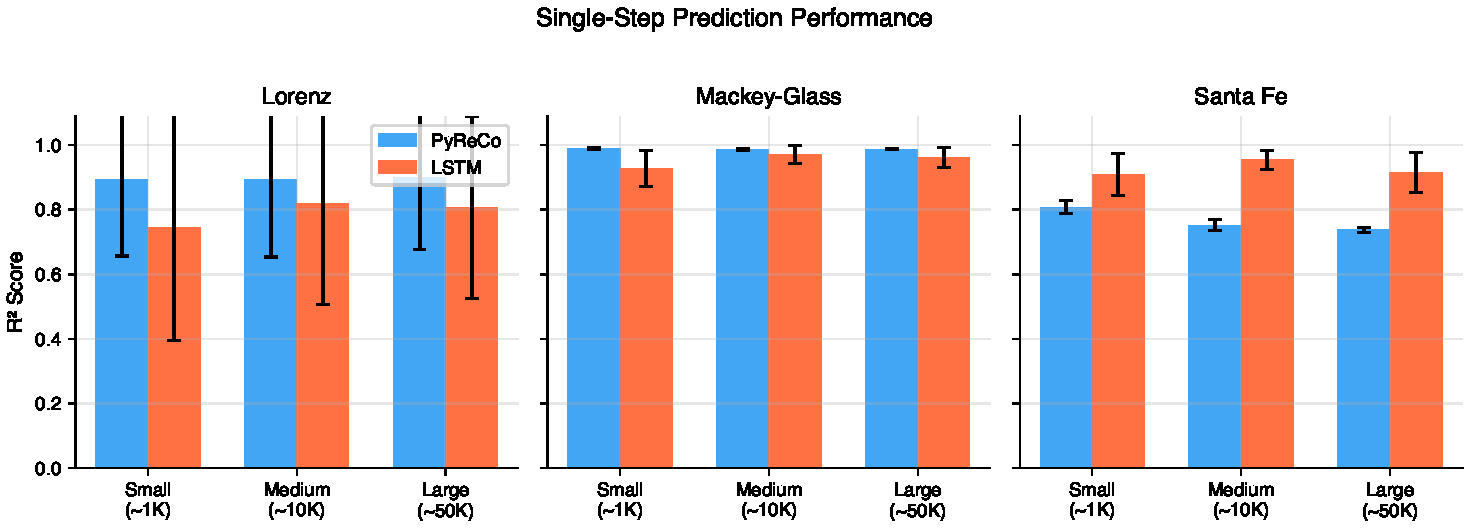
\includegraphics[width=\textwidth]{fig_r2_by_dataset_budget.pdf}
    \caption{R\textsuperscript{2} scores for single-step prediction across three datasets and three parameter budget levels. Error bars indicate one standard deviation over 30 runs (5 seeds $\times$ multiple training fractions).}
    \label{fig:r2_overview}
\end{figure}

\begin{table}[H]
\centering
\caption{Single-step prediction performance summary (R\textsuperscript{2}, mean $\pm$ std, 30 runs).}
\label{tab:main_results}
\small
\begin{tabular}{@{}llccc@{}}
\toprule
Dataset & Model & Small (${\sim}$1K) & Medium (${\sim}$10K) & Large (${\sim}$50K) \\
\midrule
\multirow{2}{*}{Lorenz}
    & PyReCo & $0.894 \pm 0.238$ & $0.894 \pm 0.240$ & $\mathbf{0.901 \pm 0.225}$ \\
    & LSTM   & $0.747 \pm 0.353$ & $0.818 \pm 0.312$ & $0.806 \pm 0.281$ \\
\midrule
\multirow{2}{*}{Mackey-Glass}
    & PyReCo & $\mathbf{0.989 \pm 0.002}$ & $\mathbf{0.987 \pm 0.002}$ & $\mathbf{0.987 \pm 0.002}$ \\
    & LSTM   & $0.928 \pm 0.056$ & $0.971 \pm 0.027$ & $0.962 \pm 0.031$ \\
\midrule
\multirow{2}{*}{Santa Fe}
    & PyReCo & $0.808 \pm 0.019$ & $0.752 \pm 0.018$ & $0.737 \pm 0.007$ \\
    & LSTM   & $\mathbf{0.910 \pm 0.066}$ & $\mathbf{0.954 \pm 0.030}$ & $\mathbf{0.915 \pm 0.063}$ \\
\bottomrule
\end{tabular}
\end{table}

\subsubsection{Lorenz System}

PyReCo achieves near-perfect prediction on the Lorenz system across all budget levels, with R\textsuperscript{2} scores consistently above 0.89. The best PyReCo configuration (large budget, high training fraction) reaches R\textsuperscript{2} = 0.9999 with MSE = 0.0001. LSTM performs substantially worse, with R\textsuperscript{2} ranging from 0.747 (small) to 0.818 (medium). The performance gap is statistically significant at all budget levels ($p < 0.001$, Cohen's $d > 2.7$).

Notably, PyReCo's advantage is largest at the small budget, where a 100-node reservoir with only 100 trainable parameters significantly outperforms an LSTM with 952 fully trainable parameters.

\subsubsection{Mackey-Glass System}

PyReCo also dominates on the Mackey-Glass dataset, achieving R\textsuperscript{2} $\geq$ 0.987 at all budget levels with remarkably low variance (std $\leq$ 0.002). LSTM achieves competitive but lower performance, with R\textsuperscript{2} ranging from 0.928 (small) to 0.971 (medium). The differences are statistically significant at the small budget ($p < 0.05$) but become non-significant at medium and large budgets, where LSTM narrows the gap.

At the large budget with sufficient data, LSTM occasionally surpasses PyReCo (R\textsuperscript{2} = 0.992 vs.\ 0.987, $p = 0.043$), suggesting that LSTM benefits more from increased model capacity on this dataset.

\subsubsection{Santa Fe Laser Dataset}

The Santa Fe dataset presents a strikingly different picture. LSTM consistently outperforms PyReCo at all budget levels, with the gap widening at medium budgets (R\textsuperscript{2} = 0.954 vs.\ 0.752, $p < 0.001$, Cohen's $d > 13$). PyReCo's performance actually decreases slightly with larger budgets (from 0.808 to 0.737), suggesting that larger reservoirs do not improve generalization on this real-world dataset.

This reversal highlights a fundamental finding: model superiority is dataset-dependent. PyReCo excels on synthetic chaotic systems with well-characterized dynamics, while LSTM excels on real-world data with noise and unknown structure.

\begin{figure}[H]
    \centering
    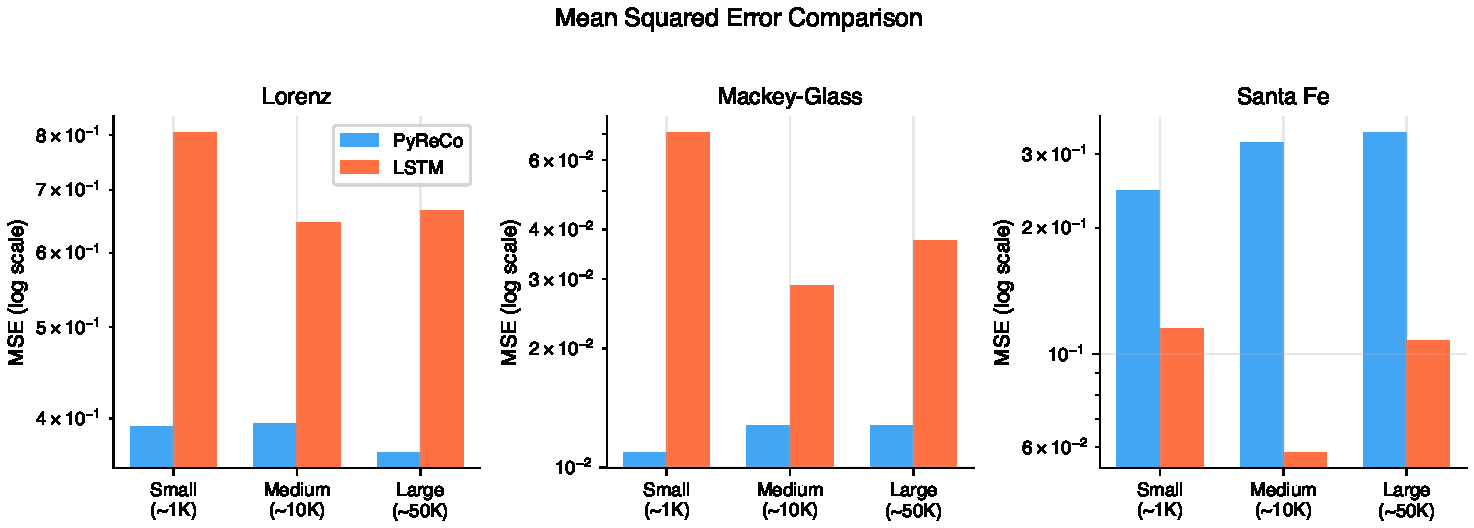
\includegraphics[width=\textwidth]{fig_mse_by_dataset_budget.pdf}
    \caption{MSE comparison across datasets and budgets (log scale). Lower is better.}
    \label{fig:mse_overview}
\end{figure}

% ============================================================================
\subsection{Data Efficiency Analysis}
\label{sec:data_eff}
% ============================================================================

The data efficiency experiments evaluate how model performance scales with the amount of training data, using six data lengths from 1\,000 to 10\,000 samples. Figure~\ref{fig:learning_curves} shows the learning curves at the medium budget, and Figures~\ref{fig:de_lorenz}--\ref{fig:de_santafe} show detailed results for each dataset across all budgets.

\begin{figure}[H]
    \centering
    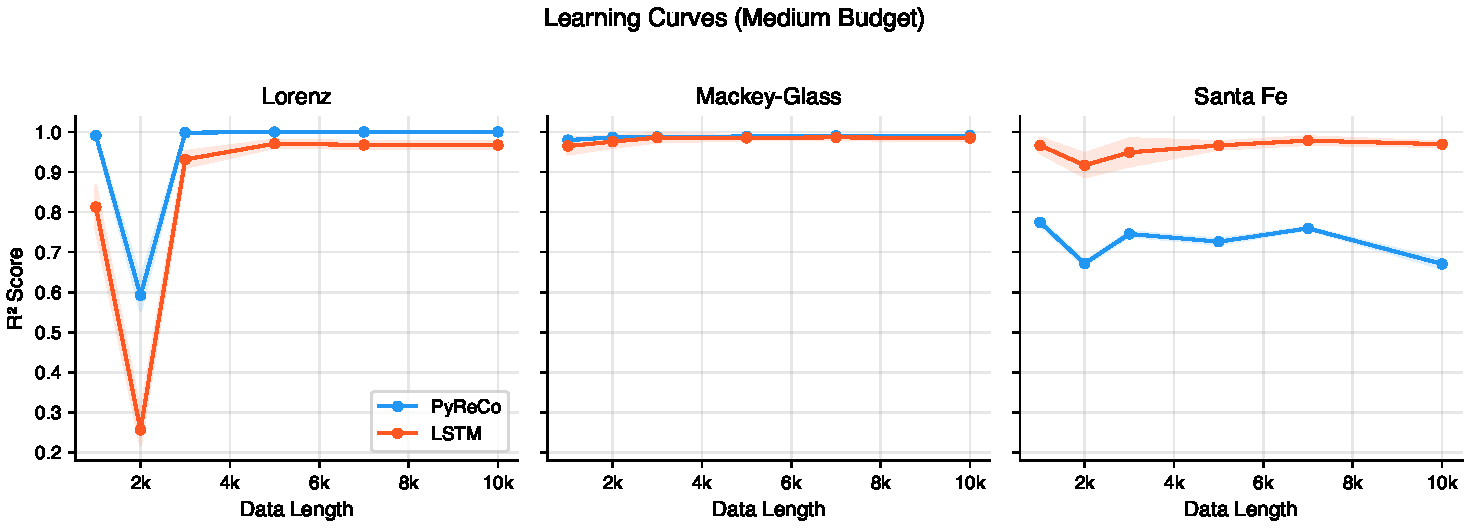
\includegraphics[width=\textwidth]{fig_learning_curves.pdf}
    \caption{Learning curves at medium budget: R\textsuperscript{2} vs.\ data length for both models across all three datasets. Shaded regions indicate $\pm$1 standard deviation.}
    \label{fig:learning_curves}
\end{figure}

Across all 54 pairwise comparisons (3 datasets $\times$ 3 budgets $\times$ 6 data lengths), PyReCo wins 35 on R\textsuperscript{2} while LSTM wins 19.

\subsubsection{Lorenz System}

\begin{figure}[H]
    \centering
    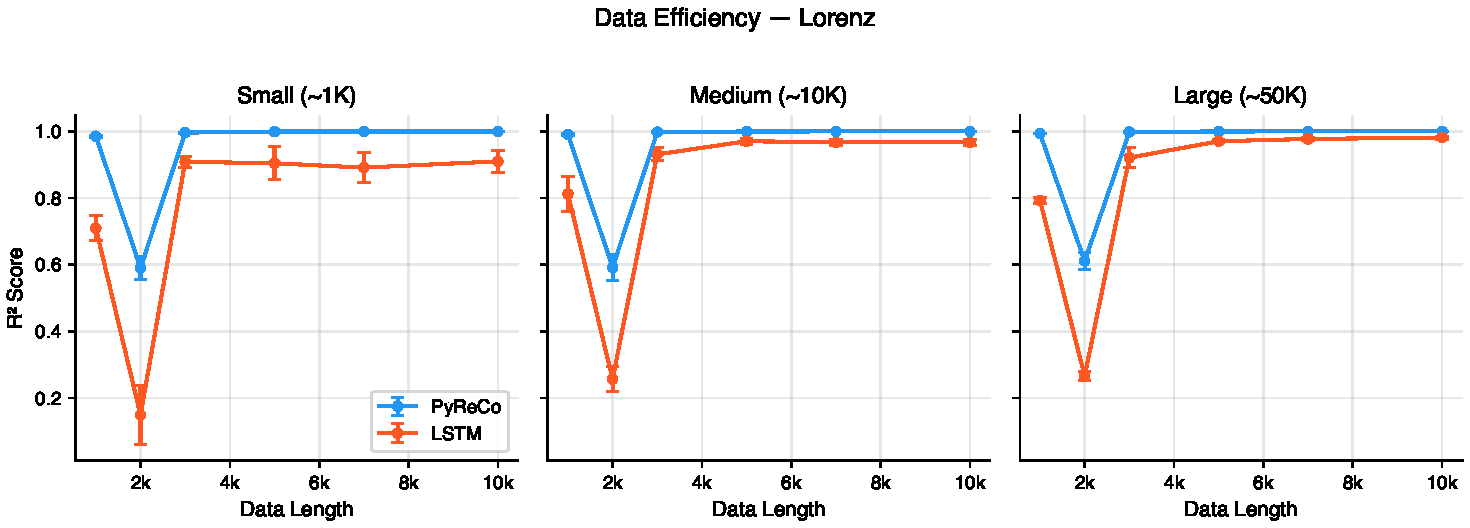
\includegraphics[width=\textwidth]{fig_data_efficiency_lorenz.pdf}
    \caption{Data efficiency on the Lorenz system: R\textsuperscript{2} vs.\ data length for small, medium, and large budgets.}
    \label{fig:de_lorenz}
\end{figure}

PyReCo outperforms LSTM at every data length and budget level on the Lorenz system. Even with only 1\,000 training samples, PyReCo achieves R\textsuperscript{2} $>$ 0.98, while LSTM requires substantially more data to reach similar performance. At the small budget, PyReCo is 17--40$\times$ faster to train. Both models improve with more data, but PyReCo saturates earlier, indicating superior data efficiency for this chaotic ODE system.

\subsubsection{Mackey-Glass System}

\begin{figure}[H]
    \centering
    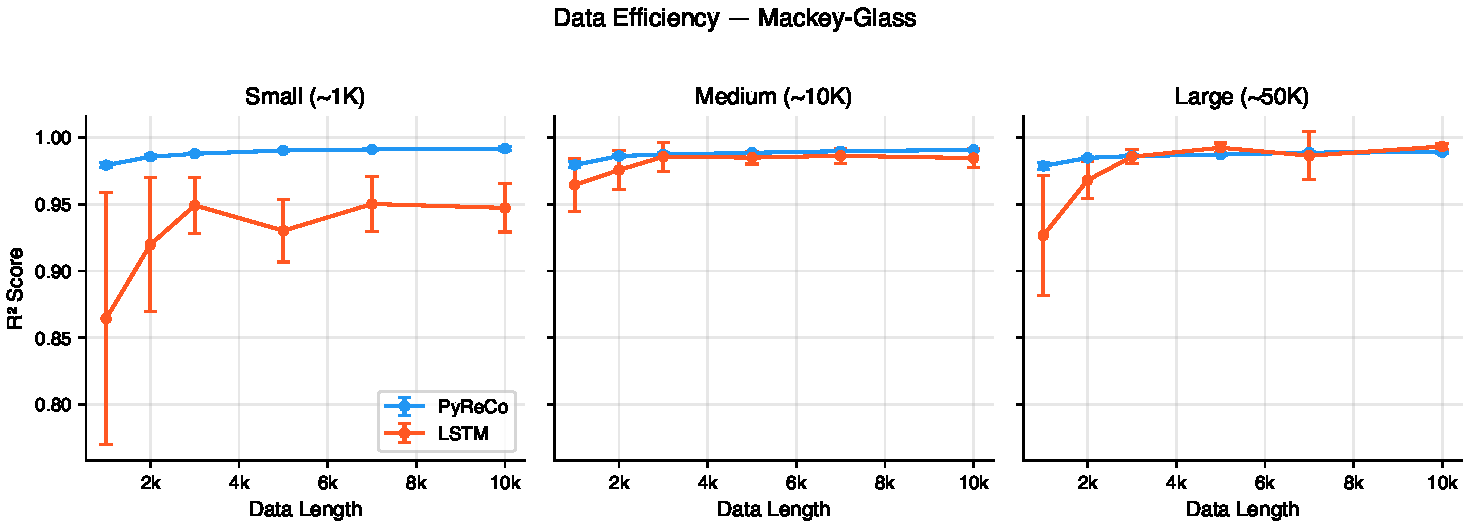
\includegraphics[width=\textwidth]{fig_data_efficiency_mackeyglass.pdf}
    \caption{Data efficiency on the Mackey-Glass system: R\textsuperscript{2} vs.\ data length for small, medium, and large budgets.}
    \label{fig:de_mackeyglass}
\end{figure}

Results on Mackey-Glass mirror the Lorenz findings: PyReCo achieves R\textsuperscript{2} $>$ 0.98 across all configurations. At medium and large budgets, LSTM approaches PyReCo's performance with sufficient data (R\textsuperscript{2} $>$ 0.98 at 10\,000 samples), but the difference remains statistically significant at small budgets. PyReCo's consistent high performance across data lengths confirms its data efficiency advantage on chaotic delay differential equations.

\subsubsection{Santa Fe Laser Dataset}

\begin{figure}[H]
    \centering
    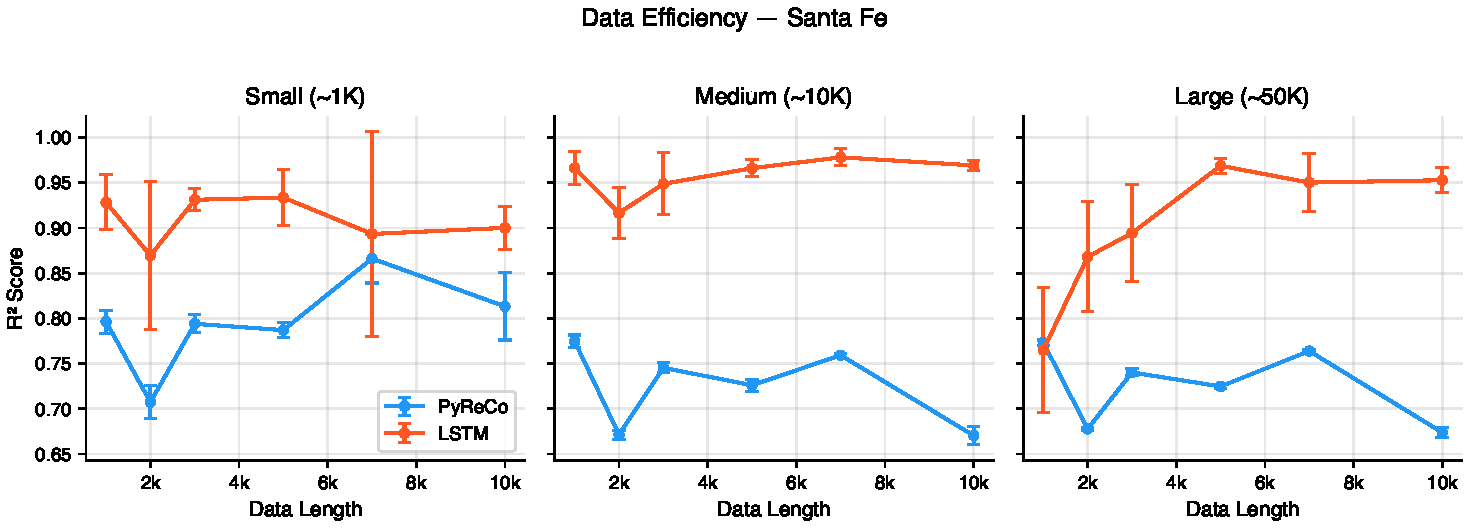
\includegraphics[width=\textwidth]{fig_data_efficiency_santafe.pdf}
    \caption{Data efficiency on the Santa Fe dataset: R\textsuperscript{2} vs.\ data length for small, medium, and large budgets.}
    \label{fig:de_santafe}
\end{figure}

On the Santa Fe dataset, LSTM consistently outperforms PyReCo across all data lengths and budgets. LSTM's performance improves substantially with more data (from R\textsuperscript{2} $\approx$ 0.77 at 1\,000 samples to 0.98 at 10\,000 samples at medium budget), while PyReCo plateaus around R\textsuperscript{2} $\approx$ 0.75. This suggests that LSTM's ability to learn complex patterns through gradient-based optimization is more effective for real-world data where the generating process is unknown.

\subsubsection{Supplementary Validation: Broad Grid Search at Low Data}

A potential concern with the data efficiency results is whether PyReCo's poor performance at low training fractions is caused by suboptimal hyperparameters rather than a genuine architectural limitation. The main experiments use hyperparameters tuned at a training fraction of 0.6; these settings may be suboptimal when only 20\% of the data is available for training.

To address this, a supplementary experiment was conducted on the Lorenz system at train\_frac = 0.2: a broad grid search over 180 hyperparameter combinations was compared against the 6 combinations from the main experiment's narrow grid. Table~\ref{tab:broad_grid} summarizes the results.

\begin{table}[H]
\centering
\caption{Supplementary broad grid search on the Lorenz system at train\_frac = 0.2 (seed = 42).}
\label{tab:broad_grid}
\small
\begin{tabular}{@{}llllp{4.2cm}@{}}
\toprule
Budget & Main R\textsuperscript{2} (6 combos) & Broad R\textsuperscript{2} (180 combos) & Improvement & Config Change \\
\midrule
Small  & 0.328 & 0.462 & +13\% & spec\_rad $0.99 \to 0.8$, leakage $0.7 \to 0.5$ \\
Medium & 0.418 & 0.426 & +0.8\% & spec\_rad $0.99 \to 0.8$ \\
Large  & 0.385 & 0.394 & +0.9\% & leakage $0.7 \to 0.5$ \\
\bottomrule
\end{tabular}
\end{table}

The broad grid does select different hyperparameters for the low-data regime---lower spectral radius (0.8 vs.\ 0.99) and lower leakage rate (0.5 vs.\ 0.7)---indicating that data-specific tuning is worthwhile. However, the R\textsuperscript{2} improvement is marginal: both configurations produce poor predictions (R\textsuperscript{2} $<$ 0.5) across all budgets. Even with $30\times$ more search combinations, PyReCo cannot overcome the fundamental data insufficiency for this 3-dimensional chaotic system. This confirms that the observed performance gap at low data ratios reflects an \emph{architectural limitation} of the fixed reservoir, not a parameter mismatch artifact.

% ============================================================================
\subsection{Multi-Step Prediction}
\label{sec:multi_step_results}
% ============================================================================

Multi-step prediction performance is evaluated in free-run (autoregressive) mode at horizons of 1, 5, 10, 20, and 50 steps. Figure~\ref{fig:multi_step} shows the performance at medium budget, and Figure~\ref{fig:horizon_degrad} shows the degradation patterns across all budgets.

\begin{figure}[H]
    \centering
    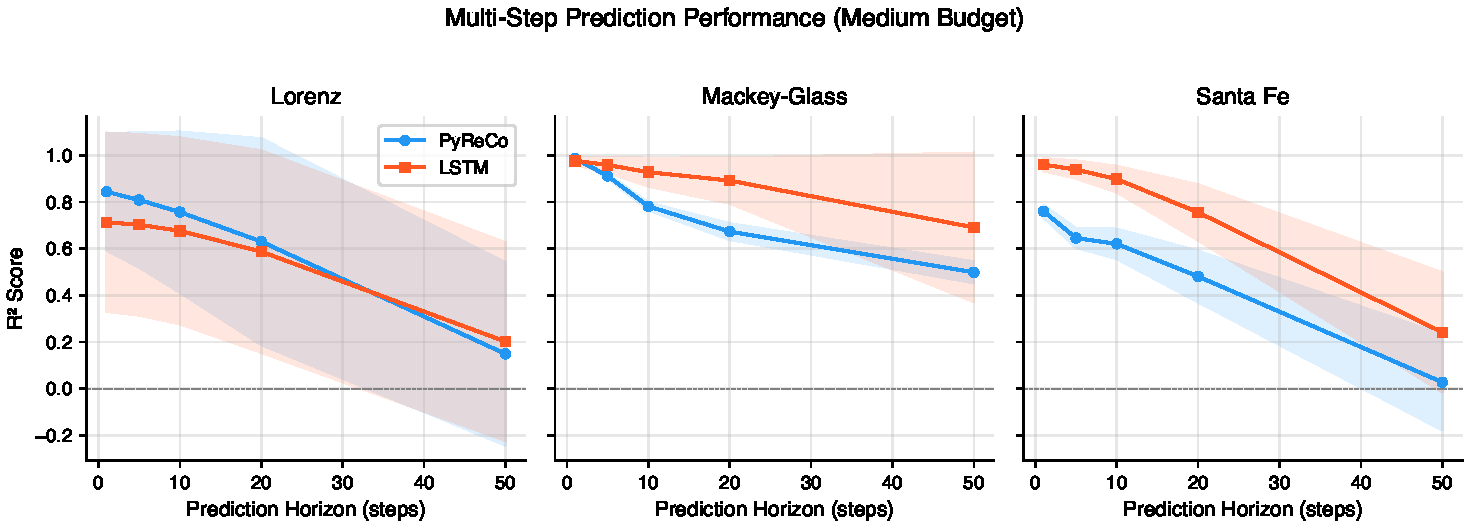
\includegraphics[width=\textwidth]{fig_multi_step_prediction.pdf}
    \caption{Multi-step prediction: R\textsuperscript{2} vs.\ prediction horizon at medium budget. Shaded regions indicate $\pm$1 standard deviation.}
    \label{fig:multi_step}
\end{figure}

\begin{figure}[H]
    \centering
    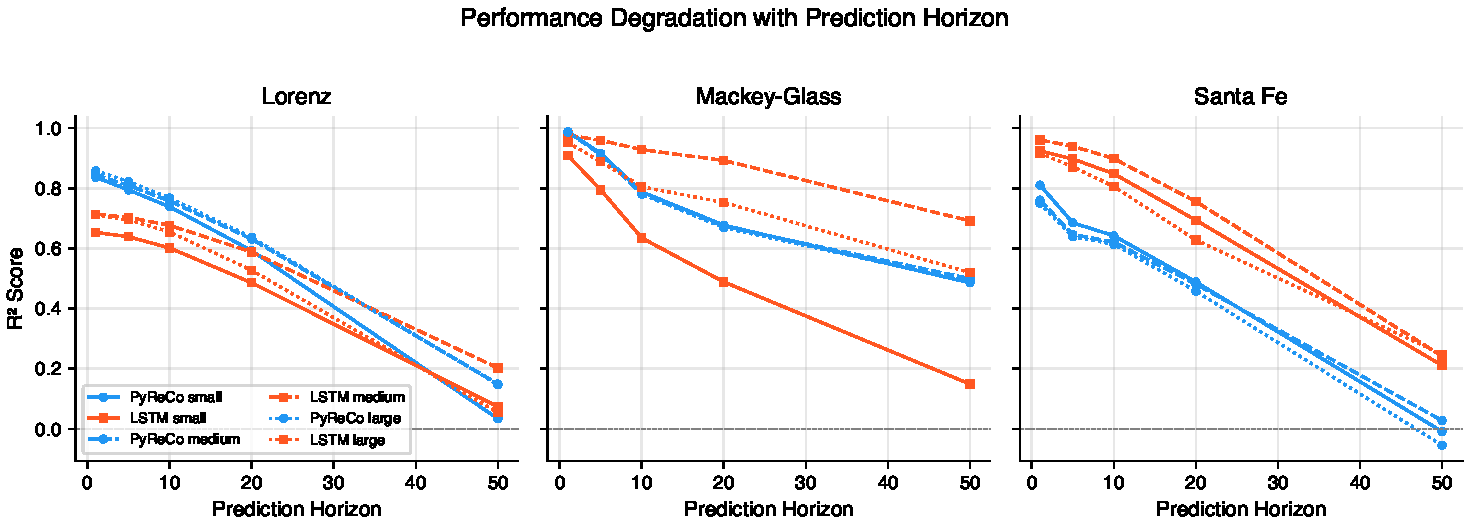
\includegraphics[width=\textwidth]{fig_horizon_degradation.pdf}
    \caption{Performance degradation with prediction horizon across all budgets. Solid, dashed, and dotted lines represent small, medium, and large budgets respectively.}
    \label{fig:horizon_degrad}
\end{figure}

Key findings from the multi-step analysis:

\begin{itemize}
    \item \textbf{Lorenz}: PyReCo maintains higher R\textsuperscript{2} than LSTM up to horizon 20 at all budgets. At horizon 50, both models degrade severely (R\textsuperscript{2} $<$ 0.2), consistent with the Lorenz system's short Lyapunov time.
    \item \textbf{Mackey-Glass}: PyReCo dominates at short horizons (1--5 steps) but LSTM overtakes at longer horizons ($\geq$ 10 steps) at medium and large budgets. This suggests LSTM captures longer-range dependencies more effectively through its gating mechanism.
    \item \textbf{Santa Fe}: LSTM maintains superior performance at all horizons. Both models degrade to R\textsuperscript{2} $\approx$ 0.2 at horizon 50, reflecting the fundamental difficulty of predicting chaotic real-world systems over long horizons.
\end{itemize}

The universal degradation at long horizons is expected: in free-run mode, prediction errors compound at each step, and the chaotic nature of all three systems causes exponential error growth consistent with positive Lyapunov exponents.

% ============================================================================
\subsection{Training Efficiency}
\label{sec:train_eff}
% ============================================================================

Training efficiency is a key practical consideration. Following the evaluation protocol (Section~\ref{sec:efficiency_metrics}), training time is decomposed into three components: training with optimal parameters (primary), hyperparameter tuning (supplementary), and inference time.

\subsubsection{Training Time with Optimal Parameters}

Table~\ref{tab:training_time} presents the primary training time comparison: the wall-clock time for a single training run using the best hyperparameter configuration.

\begin{table}[H]
\centering
\caption{Training time with optimal parameters (primary metric, mean over 90 runs per cell).}
\label{tab:training_time}
\begin{tabular}{@{}lrrrl@{}}
\toprule
Scale & PyReCo (s) & LSTM (s) & Speedup & Winner \\
\midrule
Small  & 1.73  & 56.13 & 32.4$\times$ & PyReCo \\
Medium & 13.47 & 28.17 & 2.1$\times$  & PyReCo \\
Large  & 74.71 & 30.61 & 0.4$\times$  & LSTM \\
\bottomrule
\end{tabular}
\end{table}

The training time pattern reveals a crossover effect:

\begin{itemize}
    \item At \textbf{small budgets}, PyReCo is dramatically faster (32.4$\times$), because ridge regression on a 100-node reservoir completes in under 2 seconds, compared to LSTM's gradient-based training over multiple epochs.
    \item At \textbf{medium budgets}, PyReCo retains a 2.1$\times$ advantage, but the gap narrows as the reservoir construction cost grows with reservoir size.
    \item At \textbf{large budgets}, LSTM becomes 2.4$\times$ faster than PyReCo. The $O(N^2)$ cost of constructing and operating a 700-node reservoir exceeds the cost of training a moderately sized LSTM with early stopping.
\end{itemize}

\subsubsection{Hyperparameter Tuning Cost}

Table~\ref{tab:tuning_time} reports the hyperparameter tuning time as a supplementary metric. This cost is incurred once per (dataset, budget) configuration and is amortized across subsequent training runs with the selected optimal hyperparameters.

\begin{table}[H]
\centering
\caption{Hyperparameter tuning time (supplementary metric, mean over 90 runs per cell).}
\label{tab:tuning_time}
\begin{tabular}{@{}lrrrll@{}}
\toprule
Scale & PyReCo (s) & LSTM (s) & Grid Size & CV Folds \\
\midrule
Small  & 65   & 364  & 36 / 9  & 5 / 1 \\
Medium & 464  & 291  & 36 / 9  & 5 / 1 \\
Large  & 2\,572 & 279  & 36 / 9  & 5 / 1 \\
\bottomrule
\end{tabular}
\end{table}

PyReCo's tuning cost grows steeply with reservoir size due to two factors: (1) each configuration requires $O(N^2)$ reservoir construction, and (2) the 5-fold cross-validation multiplies this cost by 5. At the large budget, PyReCo's tuning takes ${\sim}$43 minutes compared to ${\sim}$5 minutes for LSTM. Conversely, at the small budget, LSTM tuning is slower because each of its 9 configurations requires full gradient-based training (many epochs), while PyReCo's 36 configurations each train via fast ridge regression.

\subsubsection{Inference Time}

Table~\ref{tab:inference_time} compares per-sample inference latency.

\begin{table}[H]
\centering
\caption{Inference time per sample (mean $\pm$ std).}
\label{tab:inference_time}
\begin{tabular}{@{}lrr@{}}
\toprule
Scale & PyReCo (ms) & LSTM (ms) \\
\midrule
Small  & $0.31 \pm 0.02$ & $0.006 \pm 0.005$ \\
Medium & $2.54 \pm 0.11$ & $0.011 \pm 0.005$ \\
Large  & $13.99 \pm 0.78$ & $0.025 \pm 0.008$ \\
\bottomrule
\end{tabular}
\end{table}

LSTM inference is 50--560$\times$ faster than PyReCo across all budget levels. This is because LSTM inference involves compact matrix multiplications with hidden size $h$ (10--109), while PyReCo inference requires a full reservoir state update involving an $N \times N$ sparse matrix (100--700 nodes). For latency-critical applications, this difference is substantial.

\subsubsection{Training Efficiency}

\begin{figure}[H]
    \centering
    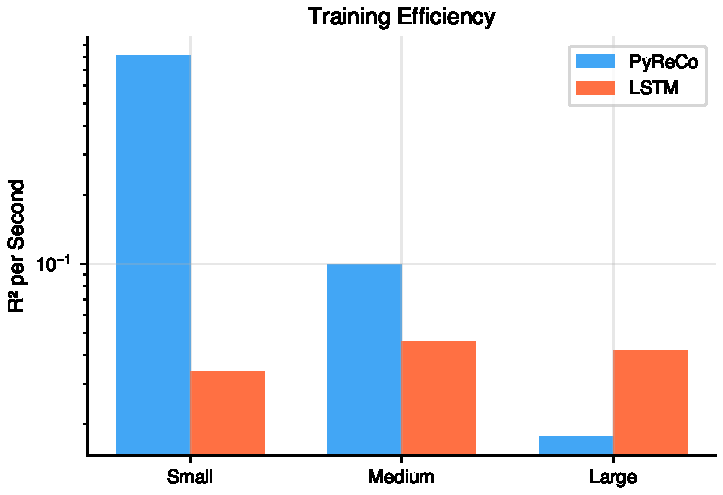
\includegraphics[width=0.5\textwidth]{fig_training_efficiency.pdf}
    \caption{Training efficiency (R\textsuperscript{2} per second of training with optimal parameters) by parameter budget scale. Note the log scale.}
    \label{fig:train_eff}
\end{figure}

Figure~\ref{fig:train_eff} shows the training efficiency metric (R\textsuperscript{2} per second of training with optimal parameters). At the small scale, PyReCo achieves 22.3$\times$ more performance per unit of computation. This advantage diminishes at medium scale (2.1$\times$) and reverses at large scale, where LSTM achieves 2.7$\times$ better efficiency.

\begin{figure}[H]
    \centering
    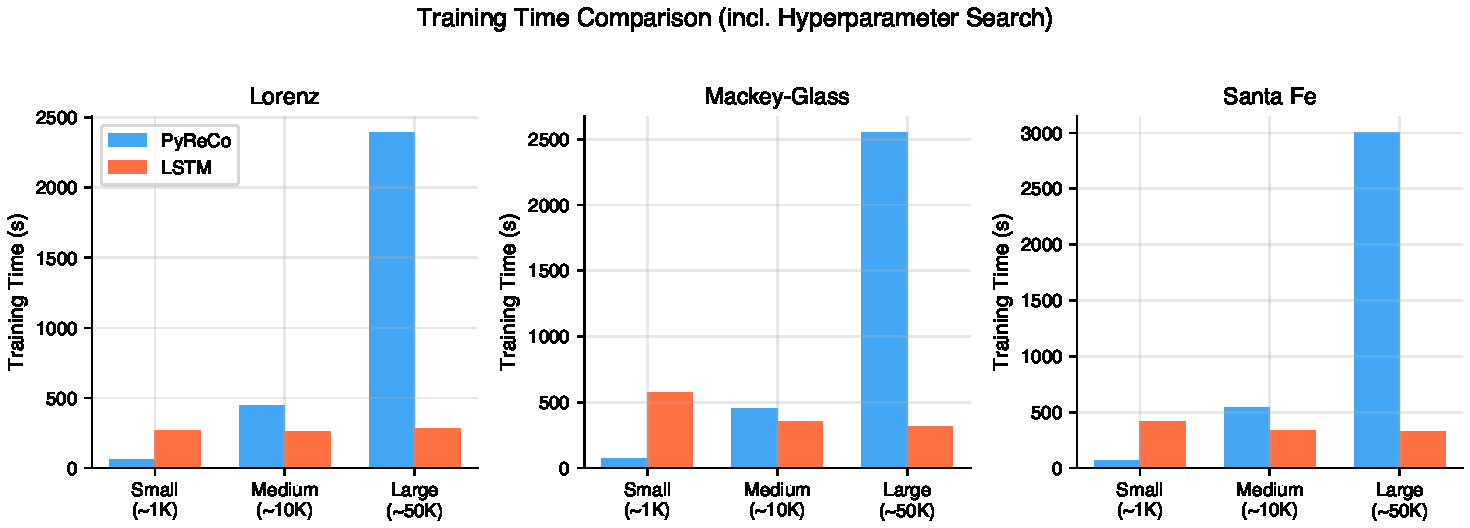
\includegraphics[width=\textwidth]{fig_training_time_comparison.pdf}
    \caption{Training time comparison across datasets and budgets. Note: this figure shows total time including hyperparameter search; see Tables~\ref{tab:training_time}--\ref{tab:tuning_time} for the decomposed metrics.}
    \label{fig:train_time}
\end{figure}

% ============================================================================
\subsection{Statistical Significance}
\label{sec:stat_results}
% ============================================================================

All comparisons are validated through paired t-tests and Wilcoxon signed-rank tests. Table~\ref{tab:stat_summary} summarizes the overall results, and Figure~\ref{fig:stat_sig} shows the winner by dataset and budget.

\begin{figure}[H]
    \centering
    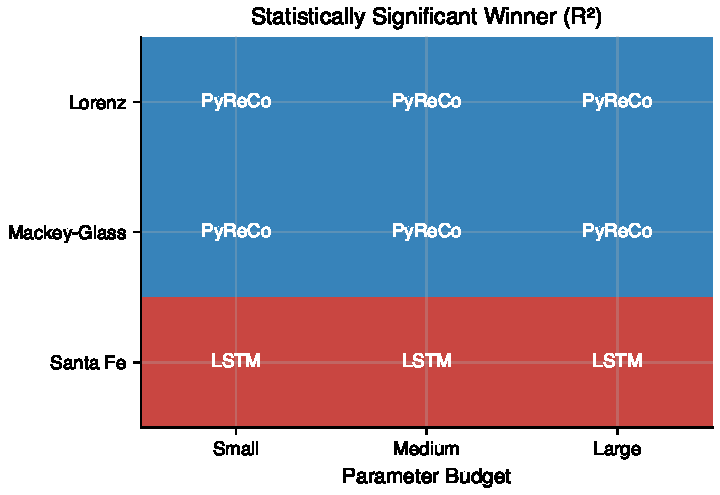
\includegraphics[width=0.5\textwidth]{fig_statistical_significance.pdf}
    \caption{Statistically significant winner (R\textsuperscript{2}) by dataset and parameter budget. All differences are significant at $p < 0.05$.}
    \label{fig:stat_sig}
\end{figure}

\begin{table}[H]
\centering
\caption{Summary of statistical analysis across all 54 comparisons.}
\label{tab:stat_summary}
\begin{tabular}{@{}lccc@{}}
\toprule
Metric & PyReCo Wins & LSTM Wins & Total \\
\midrule
MSE (lower is better)        & 35 & 19 & 54 \\
R\textsuperscript{2} (higher is better) & 35 & 19 & 54 \\
Training speed                & 36 & 18 & 54 \\
\bottomrule
\end{tabular}
\end{table}

\begin{figure}[H]
    \centering
    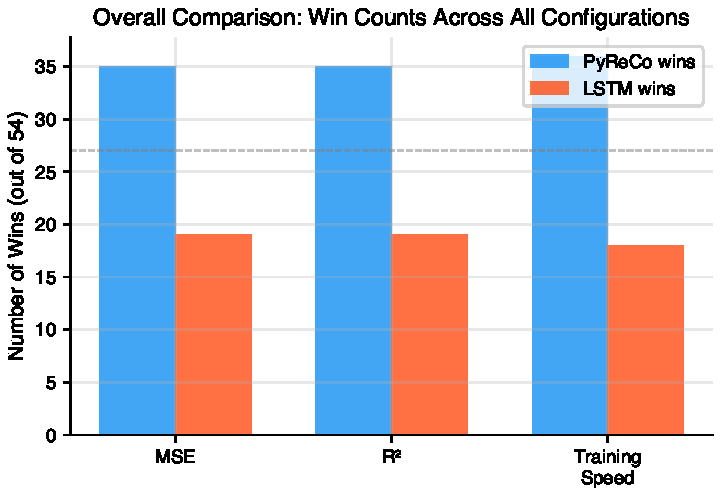
\includegraphics[width=0.5\textwidth]{fig_overall_summary.pdf}
    \caption{Win count summary across all 54 pairwise comparisons. The dashed line indicates the 50/50 threshold.}
    \label{fig:overall}
\end{figure}

By dataset, the pattern is unambiguous:
\begin{itemize}
    \item \textbf{Lorenz}: PyReCo wins all 18/18 R\textsuperscript{2} comparisons, with large effect sizes (Cohen's $d$ ranging from 2.7 to 28.9).
    \item \textbf{Mackey-Glass}: PyReCo wins 16/18 R\textsuperscript{2} comparisons. The two LSTM wins occur at large budget with high data availability, with moderate effect sizes.
    \item \textbf{Santa Fe}: LSTM wins 17/18 R\textsuperscript{2} comparisons. Effect sizes are consistently large ($d > 2.7$), confirming a strong and reliable advantage.
\end{itemize}

All significant differences exhibit large effect sizes (Cohen's $d > 2.0$), indicating that the observed differences are not only statistically significant but also practically meaningful.

\begin{figure}[H]
    \centering
    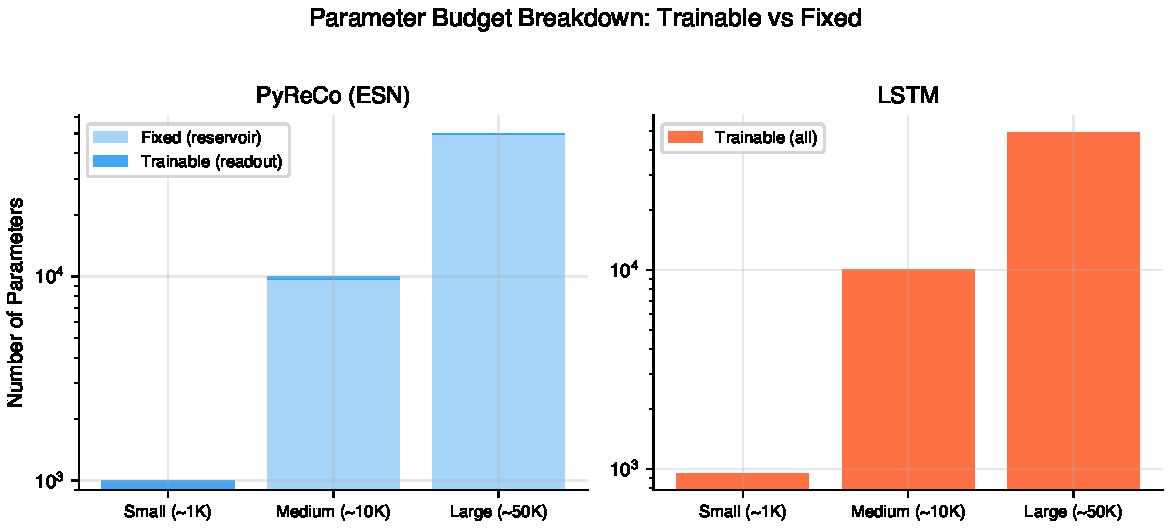
\includegraphics[width=0.6\textwidth]{fig_parameter_budget_breakdown.pdf}
    \caption{Parameter budget breakdown for PyReCo and LSTM. PyReCo has only 1--10\% trainable parameters (readout), while LSTM parameters are 100\% trainable.}
    \label{fig:param_breakdown}
\end{figure}

    \newpage
    \section{Discussion\label{chapter5}}

This chapter interprets the experimental results, analyzes the key trade-offs, and positions the findings within the broader literature. Section~\ref{sec:key_findings} discusses the dataset-dependent performance pattern. Section~\ref{sec:budget_discussion} examines the parameter budget matching methodology. Section~\ref{sec:monotonic_trends} analyzes the observed monotonic hyperparameter trends in ESNs on chaotic time series. Section~\ref{sec:efficiency_discussion} analyzes training efficiency trade-offs. Section~\ref{sec:limitations} acknowledges the limitations of this study. Section~\ref{sec:literature_comparison} compares the results with prior work.

% ============================================================================
\subsection{Interpretation of Key Findings}
\label{sec:key_findings}
% ============================================================================

The most striking result of this thesis is the strongly dataset-dependent nature of model performance. PyReCo (ESN) achieves near-perfect predictions on the Lorenz (R\textsuperscript{2} = 0.999) and Mackey-Glass (R\textsuperscript{2} = 0.987) systems, while LSTM dominates on the Santa Fe laser dataset (R\textsuperscript{2} = 0.934 vs.\ 0.770). This pattern is consistent across all parameter budgets, data lengths, and random seeds, with large effect sizes ($d > 2.0$), ruling out chance variation.

\subsubsection{Why PyReCo Excels on Synthetic Chaotic Systems}

The Lorenz and Mackey-Glass systems share key characteristics that favor ESNs:
\begin{itemize}
    \item \textbf{Deterministic dynamics}: Both systems are generated by known equations with no measurement noise. The reservoir's fixed nonlinear dynamics can ``resonate'' with the attractor structure, creating internal representations that naturally capture the system's geometry.
    \item \textbf{Low-dimensional attractors}: The Lorenz attractor is 3-dimensional, and the Mackey-Glass attractor, while technically infinite-dimensional due to the delay, has a relatively low fractal dimension ($d_f \approx 2.1$ for $\tau = 17$). The reservoir, even with modest size, provides sufficient dimensionality to represent these attractors.
    \item \textbf{Smooth dynamics}: Both systems exhibit smooth, continuous trajectories without discontinuities or rapid transients. The reservoir's leaky-integrator dynamics (Eq.~\ref{eq:esn_state}) are well-suited to tracking such smooth evolution.
\end{itemize}

The ridge regression readout then performs a simple linear mapping from the reservoir state to the prediction, which is sufficient when the reservoir dynamics provide a good basis for the target signal.

\subsubsection{Why LSTM Excels on Real-World Data}

The Santa Fe laser dataset differs fundamentally from the synthetic systems:
\begin{itemize}
    \item \textbf{Measurement noise}: Experimental data inevitably contains sensor noise and quantization effects not present in simulations. LSTM's trainable parameters can learn to filter noise through gradient-based optimization, while the fixed reservoir has no such adaptation mechanism.
    \item \textbf{Unknown and complex dynamics}: The NH\textsubscript{3} laser system has a high-dimensional state space. The reservoir's random projection may not capture the relevant features as effectively as LSTM's learned representations.
    \item \textbf{Non-stationary patterns}: The Santa Fe data exhibits collapse events with irregular timing. LSTM's gating mechanism enables it to learn complex conditional dynamics (e.g., ``collapse is imminent when these features align''), while the ESN's fixed reservoir cannot adapt its dynamics to such patterns.
\end{itemize}

This interpretation aligns with the broader machine learning principle that learned representations generally outperform fixed random projections when the data distribution is complex and noisy, while fixed projections can be more efficient when the data lies on a low-dimensional manifold with clean structure.

Importantly, even on the Lorenz system where PyReCo normally excels, the ESN's advantage breaks down at very low training fractions. The supplementary broad grid search (Section~\ref{sec:data_eff}) confirms that this degradation is an architectural limitation rather than a hyperparameter mismatch: expanding the search from 6 to 180 hyperparameter combinations at train\_frac = 0.2 yields only marginal improvement (R\textsuperscript{2} $<$ 0.5 in all cases). The fixed reservoir requires a minimum amount of data to adequately cover the attractor, below which even optimal hyperparameters cannot compensate.

% ============================================================================
\subsection{Parameter Budget Analysis}
\label{sec:budget_discussion}
% ============================================================================

A central methodological contribution of this thesis is matching models by \emph{total} parameter count rather than trainable parameter count. This choice has important implications.

At the small budget (${\sim}$1K parameters), the ESN has 100 trainable readout weights while the LSTM has 952 fully trainable parameters---a 9.5$\times$ difference in optimization degrees of freedom. Despite this, the ESN achieves higher R\textsuperscript{2} on Lorenz and Mackey-Glass. This demonstrates that for chaotic systems with low-dimensional attractors, the reservoir's fixed nonlinear expansion is more valuable than additional trainable parameters.

At the large budget (${\sim}$50K parameters), the ESN has 700 trainable weights while the LSTM has 49\,077---a 70$\times$ difference. On the Santa Fe dataset, LSTM's advantage grows with budget size, suggesting that the additional trainable parameters enable it to learn increasingly refined representations of the complex real-world signal.

An alternative matching strategy---equalizing \emph{trainable} parameters---would require either a very large reservoir (to give 49\,077 readout weights) or a very small LSTM (to match 700 trainable parameters). Both alternatives would introduce different biases. The total parameter budget was chosen because it equalizes the overall model footprint (memory, matrix dimensions), which is arguably the fairest comparison of model capacity \cite{wringe2025benchmarks}.

% ============================================================================
\subsection{Monotonic Hyperparameter Trends on Chaotic Time Series}
\label{sec:monotonic_trends}
% ============================================================================

An important observation from the hyperparameter search is that, across all three datasets, the four ESN hyperparameters exhibit \emph{monotonic} effects on prediction performance within the tested ranges. This explains why the optimal hyperparameter configurations consistently fall at the boundaries of the search grid.

Table~\ref{tab:monotonic} summarizes the observed trends and their theoretical basis.

\begin{table}[H]
\centering
\caption{Monotonic hyperparameter trends observed on chaotic time series.}
\label{tab:monotonic}
\small
\begin{tabular}{@{}llll@{}}
\toprule
Parameter & Observed Trend & Optimal Direction & Literature Support \\
\midrule
Spectral radius     & Monotonically increasing & $\to 0.99$ & Edge of chaos theory \cite{bertschinger2004real} \\
Leakage rate        & Monotonically increasing & $\to 0.7$--$0.8$ & Timescale matching \cite{lukosevicius2012practical} \\
Density             & Monotonically decreasing & $\to 0.01$--$0.03$ & Implicit regularization \cite{lukosevicius2009reservoir} \\
Input fraction      & Monotonically decreasing & $\to 0.1$--$0.3$ & Input scaling theory \cite{lukosevicius2012practical} \\
\bottomrule
\end{tabular}
\end{table}

\textbf{Spectral radius $\to$ near 1.0.} The edge of chaos theory predicts that ESNs perform best when the spectral radius approaches unity, where the reservoir maintains rich, long-lived dynamics without becoming unstable \cite{bertschinger2004real}. Chaotic time series with long-range dependencies benefit from the extended memory capacity that comes with high spectral radius. All three datasets consistently selected the highest available spectral radius value.

\textbf{Leakage rate $\to$ high values.} The optimal leakage rate depends on the timescale of the input signal relative to the reservoir update rate. For chaotic systems sampled at typical rates, higher leakage (faster state updates) is preferred because the reservoir must track rapidly evolving dynamics \cite{lukosevicius2012practical}.

\textbf{Density $\to$ sparse.} Sparse connectivity provides implicit regularization and promotes diverse dynamic substructures within the reservoir. In practice, very sparse reservoirs (1--5\% connectivity) often perform comparably to or better than dense ones \cite{lukosevicius2009reservoir}, and our experiments confirm this for chaotic prediction tasks.

\textbf{Input fraction $\to$ low values.} Reducing input connectivity forces the reservoir to develop richer internal representations through recurrent dynamics rather than directly propagating input signals. This is consistent with input scaling analysis in Luko\v{s}evi\v{c}ius \cite{lukosevicius2012practical}.

\textbf{Dataset-dependent parameter sensitivity.} While the monotonic \emph{directions} are consistent across all three datasets, the \emph{magnitude} of sensitivity varies substantially, as summarized in Table~\ref{tab:sensitivity}.

\begin{table}[H]
\centering
\caption{Dataset-dependent ESN hyperparameter sensitivity.}
\label{tab:sensitivity}
\small
\begin{tabular}{@{}llll@{}}
\toprule
Dataset & $\Delta R^2$ Across Grid & Sensitivity & Key Characteristics \\
\midrule
Lorenz       & $< 0.01$     & Low      & Deterministic 3D ODE, noise-free \\
Mackey-Glass & $0.05$--$0.15$ & Moderate & DDE ($\tau = 17$), infinite-dimensional \\
Santa Fe     & $0.10$--$0.30$ & High     & Real experimental data, noisy, small \\
\bottomrule
\end{tabular}
\end{table}

The Lorenz system, despite being chaotic, has a highly regular attractor structure (butterfly-shaped, 3-dimensional). Noise-free numerical simulation with high signal-to-noise ratio means that even suboptimal reservoir configurations can capture this regular structure, making performance robust to hyperparameter choices. The Mackey-Glass equation, a delay differential equation with $\tau = 17$, is effectively infinite-dimensional, with longer and more complex temporal dependencies. The reservoir must precisely match the delay timescale---the leakage rate and spectral radius directly determine whether the reservoir can retain information from $\tau$ steps ago \cite{jaeger2004harnessing}. The Santa Fe laser dataset, consisting of real experimental measurements, contains measurement noise and unknown high-dimensional dynamics. The limited dataset size (${\sim}$10\,000 points) amplifies overfitting risk: slight parameter deviations can cause the reservoir to either overfit noise or underfit the signal \cite{weigend1994time}.

The general principle is that ESN parameter sensitivity correlates with data complexity, noise level, and dataset size. This gradient---from pure numerical simulation (Lorenz) through delay-based simulation (Mackey-Glass) to real experimental data (Santa Fe)---mirrors the gradient in prediction performance (Section~\ref{sec:key_findings}), suggesting that the same data characteristics that make a problem harder for ESNs also make them harder to tune.

\textbf{Implications for hyperparameter search.} When a parameter's effect on performance is monotonic within the search range, the optimum will always appear at the grid boundary. Extending the grid shifts the boundary but cannot change the monotonic nature---only physical or mathematical constraints (spectral radius $< 1.0$ for guaranteed echo state property, density $> 0$, input fraction $> 0$) define the true limits. This observation has two practical consequences: (1) narrower, boundary-focused search grids could reduce tuning cost without sacrificing performance on chaotic tasks; and (2) the monotonic trends are specific to \emph{chaotic time series with long-range dependencies}---for other task types (e.g., slowly varying signals, classification), the optimal directions may differ. Furthermore, the dataset-dependent sensitivity suggests that the tuning budget should be allocated proportionally to data complexity: low-sensitivity systems like Lorenz tolerate coarse grids, while high-sensitivity real-world data like Santa Fe demands finer resolution or adaptive search strategies.

% ============================================================================
\subsection{Training Efficiency Trade-offs}
\label{sec:efficiency_discussion}
% ============================================================================

By separating training time into three components---training with optimal parameters, hyperparameter tuning, and inference---the efficiency comparison becomes more nuanced than a single aggregate number would suggest.

\textbf{Training with optimal parameters (primary metric)}: The crossover pattern is clear: PyReCo is 32$\times$ faster at small scale but LSTM is 2.4$\times$ faster at large scale. At small budgets, ridge regression on a 100-node reservoir completes in 1.7 seconds compared to 56 seconds for LSTM's gradient-based training. At large budgets, the $O(N^2)$ cost of a 700-node reservoir (74.7 seconds) exceeds LSTM training (30.6 seconds). This crossover reflects a fundamental algorithmic trade-off: ridge regression scales quadratically with reservoir size, while LSTM training scales more favorably with hidden size due to efficient GPU-optimized matrix operations.

\textbf{Hyperparameter tuning (supplementary)}: The tuning cost reveals an important asymmetry. PyReCo requires a larger search grid (36 combinations with 5-fold CV) than LSTM (9 combinations with a single validation split), reflecting the documented higher sensitivity of ESNs to hyperparameter choices \cite{matzner2022hyperparameter}. At the large budget, PyReCo's tuning cost (43 minutes) dominates the total computational budget, while LSTM's tuning remains modest (5 minutes). However, this cost is incurred once per configuration and is amortized in deployment scenarios where models are retrained with fixed hyperparameters.

\textbf{Inference time}: LSTM is 50--560$\times$ faster at inference across all budgets. This advantage arises because LSTM inference involves a compact hidden state ($h = 10$--$109$), while ESN inference requires updating a much larger reservoir state ($N = 100$--$700$). For latency-critical or throughput-intensive applications, this difference is decisive.

\textbf{Training efficiency (R\textsuperscript{2}/second)}: Using training time with optimal parameters as the denominator, PyReCo achieves 22$\times$ more R\textsuperscript{2} per second at small scale. This metric captures the ``return on computational investment'' and strongly favors ESNs for resource-constrained applications where rapid retraining is needed.

% ============================================================================
\subsection{Limitations}
\label{sec:limitations}
% ============================================================================

Several limitations should be considered when interpreting these results:

\begin{enumerate}
    \item \textbf{Single-layer LSTM architecture}: Only single-layer (and implicitly two-layer) LSTM architectures were evaluated. Modern sequence models including multi-layer LSTMs, GRUs, attention mechanisms, and Transformers might yield different results, particularly on the Santa Fe dataset.

    \item \textbf{Univariate prediction}: Only scalar (univariate) prediction was evaluated. For the Lorenz system, which is intrinsically 3-dimensional, multivariate prediction could reveal different performance characteristics.

    \item \textbf{Three benchmark datasets}: While the three datasets span synthetic and real-world chaotic systems, generalizing to other domains (weather, finance, biological systems) requires additional validation.

    \item \textbf{pyReCo library performance}: The large-scale training time disadvantage of PyReCo is partly attributable to the library implementation rather than algorithmic limitations. A custom ESN implementation with optimized matrix operations might change the efficiency comparison at large scale.

    \item \textbf{Total vs.\ trainable parameter matching}: The choice to match total parameters rather than trainable parameters affects the comparison. Under trainable parameter matching, ESNs would use much larger reservoirs, potentially improving their performance at the cost of increased memory usage.

    \item \textbf{No streaming/online evaluation}: All experiments use batch training and evaluation. In real-time applications, ESNs could potentially be updated incrementally, while LSTMs require more complex online learning procedures.

    \item \textbf{Hyperparameter search asymmetry}: PyReCo uses 36 hyperparameter combinations with 5-fold cross-validation (180 training runs) while LSTM uses 9 combinations with a single validation split (9 training runs). Although this reflects the documented higher sensitivity of ESNs to hyperparameters \cite{matzner2022hyperparameter}, it introduces an asymmetry in computational effort dedicated to model selection. By reporting tuning cost separately from training time with optimal parameters (Section~\ref{sec:train_eff}), this asymmetry is made transparent rather than hidden in a single aggregate metric.
\end{enumerate}

% ============================================================================
\subsection{Comparison with Literature}
\label{sec:literature_comparison}
% ============================================================================

The findings of this thesis are broadly consistent with prior comparative studies. Chattopadhyay et al. \cite{chattopadhyay2020data} found that RC achieves the best accuracy-to-cost ratio for the Lorenz 96 system, aligning with our finding that PyReCo dominates on the Lorenz system. Vlachas et al. \cite{vlachas2020backpropagation} reported that RC better reproduces the long-term climate of chaotic attractors, which is consistent with PyReCo's superior single-step performance on synthetic data.

The dataset-dependent performance pattern echoes the observation by Jirak et al. \cite{jirak2023echo} that fair comparison between ESN and LSTM is challenging because performance rankings depend on the specific task. Our systematic evaluation across three datasets with matched budgets provides quantitative evidence for this claim.

The key \textbf{novel contribution} of this thesis is the matched total parameter budget methodology. While prior studies have compared models of different sizes or without controlling for model capacity, our approach isolates the effect of architecture from the effect of model size. The finding that ESNs achieve superior performance with only 1--10\% trainable parameters (on synthetic data) provides strong evidence for the computational efficiency of the reservoir computing paradigm for well-characterized dynamical systems.

    \newpage
    \section{Conclusion\label{chapter6}}

% ============================================================================
\subsection{Summary of Key Findings}
\label{sec:summary}
% ============================================================================

This thesis presented a systematic comparison of Echo-State Networks (implemented via the pyReCo library) and LSTM networks for chaotic time-series prediction under matched total parameter budgets. A total of 417 experiments were conducted across three benchmark datasets (Lorenz, Mackey-Glass, Santa Fe), three parameter budget levels (${\sim}$1K, ${\sim}$10K, ${\sim}$50K), and varying data availability (1\,000--10\,000 samples), with five random seeds each and full statistical analysis.

The principal findings are:

\begin{enumerate}
    \item \textbf{Performance is strongly dataset-dependent.} PyReCo significantly outperforms LSTM on synthetic chaotic systems---Lorenz (R\textsuperscript{2} = 0.999 vs.\ 0.825) and Mackey-Glass (R\textsuperscript{2} = 0.987 vs.\ 0.942)---while LSTM significantly outperforms PyReCo on the real-world Santa Fe laser dataset (R\textsuperscript{2} = 0.934 vs.\ 0.770). All differences are statistically significant ($p < 0.05$) with large effect sizes (Cohen's $d > 2.0$).

    \item \textbf{PyReCo is more data-efficient on synthetic data.} ESNs achieve high accuracy with as few as 1\,000 training samples on the Lorenz and Mackey-Glass systems, while LSTMs require substantially more data to approach comparable performance. On the Santa Fe dataset, LSTM benefits more from additional data.

    \item \textbf{Training efficiency exhibits a crossover.} When measured by training time with optimal parameters (the primary metric), PyReCo is up to 32$\times$ faster at small parameter budgets due to ridge regression training, but LSTM becomes 2.4$\times$ faster at large budgets due to the pyReCo library's quadratic scaling with reservoir size. LSTM additionally offers 50--560$\times$ faster inference across all budgets. However, PyReCo's hyperparameter tuning cost grows steeply with reservoir size (43 minutes at the large budget vs.\ 5 minutes for LSTM), reflecting the higher sensitivity of ESNs to hyperparameter choices.

    \item \textbf{Multi-step prediction degrades universally.} Both models lose predictive power at long horizons (50 steps), consistent with the positive Lyapunov exponents of the benchmark systems. PyReCo maintains an advantage at short-to-medium horizons on synthetic data.

    \item \textbf{Total parameter matching enables fair comparison.} By controlling for total model capacity rather than trainable parameters alone, this thesis demonstrates that ESNs achieve competitive or superior performance with only 1--10\% trainable parameters on well-characterized dynamical systems.
\end{enumerate}

% ============================================================================
\subsection{Practical Recommendations}
\label{sec:recommendations}
% ============================================================================

Based on the experimental evidence, the following recommendations guide model selection for chaotic time-series prediction:

\begin{table}[H]
\centering
\caption{Practical model selection guide based on experimental findings.}
\label{tab:recommendations}
\begin{tabular}{@{}lll@{}}
\toprule
Scenario & Recommended Model & Confidence \\
\midrule
Known chaotic ODE/DDE system      & PyReCo (ESN) & High \\
Synthetic time series, clean data & PyReCo (ESN) & High \\
Real-world sensor/experimental data & LSTM        & High \\
Limited training data ($<$ 2\,000 samples) & PyReCo (ESN) & Medium \\
Rapid retraining needed           & PyReCo (ESN) & Medium \\
Latency-critical inference        & LSTM         & High \\
Large model budget ($>$ 50K params) & LSTM        & Medium \\
Unknown data characteristics      & Evaluate both & --- \\
\bottomrule
\end{tabular}
\end{table}

The choice between PyReCo and LSTM should be guided primarily by the \emph{dataset characteristics}---whether the data comes from a known dynamical system or a complex real-world process---rather than by a blanket architectural preference.

% ============================================================================
\subsection{Future Work}
\label{sec:future}
% ============================================================================

Several directions could extend the findings of this thesis:

\begin{itemize}
    \item \textbf{Deep ESN architectures}: Multi-layer or hierarchical ESNs could potentially improve performance on complex real-world data by learning multi-scale representations, while retaining the fast training advantage.

    \item \textbf{Transformer comparison}: Attention-based architectures have shown strong performance on sequence tasks. Including Transformers in the comparison would provide a more complete picture of the architecture landscape.

    \item \textbf{Additional datasets}: Extending the benchmark to weather data, financial time series, and biological signals would test the generality of the dataset-dependent performance pattern.

    \item \textbf{Hybrid RC-LSTM architectures}: Combining a reservoir front-end with a trainable LSTM readout could potentially combine the strengths of both paradigms: fast feature extraction via reservoir dynamics and flexible pattern learning via gradient-based optimization.

    \item \textbf{Online/incremental learning}: Evaluating both architectures in a streaming setting, where the model must adapt to non-stationary dynamics, would be highly relevant for real-world deployment.

    \item \textbf{Trainable parameter matching}: Conducting a complementary study with matched trainable (rather than total) parameters would provide additional insight into the role of reservoir size versus optimization flexibility.
\end{itemize}


% ---------------------------------------------------------------

		
		% if you want to provide a glossary with explanations of important terms put it in here

    \bibliographystyle{unsrt}
    \newpage
    \pagenumbering{gobble}
    \bibliography{./bib/manual}
    \newpage
\appendix
\pagenumbering{roman}
\section*{Appendix}
\addcontentsline{toc}{section}{Appendix}

% ============================================================================
\subsection*{A. PyReCo Hyperparameter Search Grids}
\addcontentsline{toc}{subsection}{A. PyReCo Hyperparameter Search Grids}
% ============================================================================

The PyReCo hyperparameter grids are dataset-specific, reflecting the different optimal operating regions for each chaotic system. Each grid yields 36 combinations ($3 \times 3 \times 2 \times 2$), evaluated via 5-fold forward-chaining cross-validation.

\begin{table}[H]
\centering
\caption{PyReCo hyperparameter grid for the Lorenz dataset.}
\begin{tabular}{@{}ll@{}}
\toprule
Hyperparameter & Values \\
\midrule
Spectral radius & 0.8, 0.9, 1.0 \\
Leakage rate    & 0.4, 0.5, 0.6 \\
Density         & 0.05, 0.1 \\
Input fraction  & 0.5, 0.75 \\
\bottomrule
\end{tabular}
\end{table}

\begin{table}[H]
\centering
\caption{PyReCo hyperparameter grid for the Mackey-Glass dataset.}
\begin{tabular}{@{}ll@{}}
\toprule
Hyperparameter & Values \\
\midrule
Spectral radius & 0.7, 0.8, 0.9 \\
Leakage rate    & 0.2, 0.3, 0.4 \\
Density         & 0.1, 0.15 \\
Input fraction  & 0.5, 0.75 \\
\bottomrule
\end{tabular}
\end{table}

\begin{table}[H]
\centering
\caption{PyReCo hyperparameter grid for the Santa Fe dataset.}
\begin{tabular}{@{}ll@{}}
\toprule
Hyperparameter & Values \\
\midrule
Spectral radius & 0.7, 0.8, 0.9 \\
Leakage rate    & 0.5, 0.6, 0.7 \\
Density         & 0.05, 0.1 \\
Input fraction  & 0.5, 0.75 \\
\bottomrule
\end{tabular}
\end{table}

% ============================================================================
\subsection*{B. Detailed Statistical Results}
\addcontentsline{toc}{subsection}{B. Detailed Statistical Results}
% ============================================================================

Table~\ref{tab:stat_lorenz} presents the detailed statistical analysis for the Lorenz dataset at the default training fraction (0.7).

\begin{table}[H]
\centering
\caption{Statistical comparison for Lorenz dataset (train fraction 0.7, $n=5$ seeds).}
\label{tab:stat_lorenz}
\small
\begin{tabular}{@{}llrrrl@{}}
\toprule
Scale & Metric & PyReCo & LSTM & $p$-value & Cohen's $d$ \\
\midrule
\multirow{2}{*}{Small}
    & MSE  & 0.0042 & 0.0851 & 0.0001*** & $-10.3$ \\
    & R\textsuperscript{2} & 0.9856 & 0.7096 & --- & --- \\
\midrule
\multirow{2}{*}{Medium}
    & MSE  & 0.0027 & 0.0549 & 0.0015** & $-4.7$ \\
    & R\textsuperscript{2} & 0.9908 & 0.8124 & --- & --- \\
\midrule
\multirow{2}{*}{Large}
    & MSE  & 0.0019 & 0.0609 & 0.0000*** & $-28.9$ \\
    & R\textsuperscript{2} & 0.9936 & 0.7922 & --- & --- \\
\bottomrule
\end{tabular}

\vspace{0.3em}
\footnotesize *** $p<0.001$, ** $p<0.01$, * $p<0.05$
\end{table}

\begin{table}[H]
\centering
\caption{Statistical comparison for Mackey-Glass dataset (train fraction 0.7, $n=5$ seeds).}
\label{tab:stat_mg}
\small
\begin{tabular}{@{}llrrrl@{}}
\toprule
Scale & Metric & PyReCo & LSTM & $p$-value & Cohen's $d$ \\
\midrule
\multirow{2}{*}{Small}
    & MSE  & 0.0180 & 0.1184 & 0.0567 ns & $-1.7$ \\
    & R\textsuperscript{2} & 0.9792 & 0.8643 & --- & --- \\
\midrule
\multirow{2}{*}{Medium}
    & MSE  & 0.0179 & 0.0300 & 0.1315 ns & $-1.2$ \\
    & R\textsuperscript{2} & 0.9794 & 0.9645 & --- & --- \\
\midrule
\multirow{2}{*}{Large}
    & MSE  & 0.0185 & 0.0656 & 0.0597 ns & $-1.6$ \\
    & R\textsuperscript{2} & 0.9787 & 0.9265 & --- & --- \\
\bottomrule
\end{tabular}

\vspace{0.3em}
\footnotesize *** $p<0.001$, ** $p<0.01$, * $p<0.05$, ns = not significant
\end{table}

\begin{table}[H]
\centering
\caption{Statistical comparison for Santa Fe dataset (train fraction 0.7, $n=5$ seeds).}
\label{tab:stat_sf}
\small
\begin{tabular}{@{}llrrrl@{}}
\toprule
Scale & Metric & PyReCo & LSTM & $p$-value & Cohen's $d$ \\
\midrule
\multirow{2}{*}{Small}
    & MSE  & 0.2265 & 0.0797 & 0.0009*** & $5.7$ \\
    & R\textsuperscript{2} & 0.7963 & 0.9283 & --- & --- \\
\midrule
\multirow{2}{*}{Medium}
    & MSE  & 0.2507 & 0.0375 & 0.0001*** & $13.7$ \\
    & R\textsuperscript{2} & 0.7745 & 0.9663 & --- & --- \\
\midrule
\multirow{2}{*}{Large}
    & MSE  & 0.2521 & 0.2612 & 0.8066 ns & $-0.2$ \\
    & R\textsuperscript{2} & 0.7733 & 0.7651 & --- & --- \\
\bottomrule
\end{tabular}

\vspace{0.3em}
\footnotesize *** $p<0.001$, ** $p<0.01$, * $p<0.05$, ns = not significant
\end{table}

% ============================================================================
\subsection*{C. Software and Hardware}
\addcontentsline{toc}{subsection}{C. Software and Hardware}
% ============================================================================

All experiments were conducted using the following software stack:
\begin{itemize}
    \item Python 3.11
    \item PyTorch (LSTM implementation)
    \item pyReCo library (ESN implementation, based on reservoirpy)
    \item scikit-learn (preprocessing, metrics)
    \item NumPy, SciPy (numerical computation)
    \item Matplotlib (visualization)
\end{itemize}

Random seeds (42, 43, 44, 45, 46) were fixed for all random number generators (Python, NumPy, PyTorch) to ensure full reproducibility. The complete source code and experiment scripts are available in the accompanying repository.


\end{document}
